\documentclass[a4paper, french, 12pt, titlepage]{article}
\usepackage[latin1, utf8]{inputenc}
\usepackage[T1]{fontenc}
\usepackage{graphicx,  amsmath, amssymb}
\renewcommand{\contentsname}{Sommaire}
\usepackage[margin = 1in]{geometry}
\graphicspath{{./images/}}
\usepackage{float}
\usepackage{appendix}
\usepackage{hyperref}
\usepackage{pdfpages}
\usepackage{fullpage}
\hypersetup{pdfnewwindow}
%\renewcommand{\appendixpagename}{Annexes}
%\renewcommand{\appendixtocname}{Annexes}

\newcommand{\HRule}{\rule{\linewidth}{0.5mm}}
\newcommand{\blap}[1]{\vbox to 0pt{#1\vss}}
\newcommand\AtUpperLeftCorner[3]{%
   \put(\LenToUnit{#1}, \LenToUnit{\dimexpr\paperheight-#2}){\blap{#3}}%
}
\newcommand\AtUpperRightCorner[3]{%
   \put(\LenToUnit{\dimexpr\paperwidth-#1}, \LenToUnit{\dimexpr\paperheight-#2}){\blap{\llap{#3}}}%
}   
   
   
\title{\LARGE{Rapport de stage\\ \ \\\textbf{Modélisation numérique d’oscillateurs non-linéaires pour la récupération d’énergie vibratoire}}} 
\author{\\ \ \\ \ \\ \textsc{LÉGLISE} Cloé\\Polytech Annecy-Chambéry - SNI4\\Année universitaire 2022/2023 \\ \ \\ \ \\Tutrice de stage\\\textsc{SAINT-MARTIN} Camille\\ \ \\ \ \\Tuteur école\\\textsc{ATTO} Abdourrahmane}
\makeatletter

\begin{document}

\begin{titlepage}
\enlargethispage{2cm}
\AddToShipoutPicture{
	\AtUpperLeftCorner{1.5cm}{1cm}{
\includegraphics[width = 6cm, height = 2cm]{logo}}
	\AtUpperRightCorner{1.5cm}{1cm}{
\includegraphics[width = 5cm, height = 2cm]{symme}}
}
\begin{center}
   \vspace*{6cm}
   \textsc{\@title}
   \HRule
   \vspace*{0.5cm}
   \large{\@author}
\end{center}
  \vspace*{2cm}
\end{titlepage}
\ClearShipoutPicture


\begin{center}
Je tiens à remercier Camille SAINT-MARTIN, ma tutrice de stage, pour m'avoir offert cette opportunité et m'avoir épaulée durant la totalité de ce stage. \\
\end{center}

\begin{center}
Je souhaite également remercier Ludovic CHARLEUX, directeur de thèse de Camille SAINT-MARTIN, sans qui ce stage n'aurait pas été possible. \\
\end{center}

\begin{center}
Je suis aussi reconnaissante envers Abdourrahmane ATTO d'avoir pris le temps, en tant que tuteur école, de rechercher et m'envoyer des ressources, alors que ce n'était pas dans ses obligations. 
\end{center}



\newpage

\section*{Résumé}


Ce stage a été réalisé dans le cadre d'un projet de recherche sur la récupération d'énergie vibratoire. 
Les récupérateurs d'énergie pourraient être une alternative plus propre aux batteries au lithium, à durée de vie limitée et très polluantes. Le but de ce stage est de réaliser une application avec interface graphique permettant de modéliser le comportement d'oscillateurs mécaniques et de pouvoir observer en temps réel l'impact de certains paramètres sur ceux-ci. 
Cette application a été réalisée en Julia, un langage informatique particulièrement adapté puisqu'il permet de créer des animations de façon facile et intuitive. Au moment de la rédaction de ce rapport, l'application n'est pas encore terminée. 
Le plus gros de ce stage a consisté en la recherche d'outils les plus adaptés possibles et la maîtrise du langage Julia. Les deux semaines de stage restantes seront donc consacrées à l'assemblage des différents éléments afin de créer une application cohérente, qui consistera en une fenêtre principale permettant de lancer différentes animations. 



\section*{Mots-clefs}

Récupération d'énergie vibratoire, modélisation, analyse numérique, dynamique non-linéaire, développement d'application.

\newpage 

\tableofcontents

\newpage 



\section{Introduction}

Alors que les enjeux climatiques deviennent de plus en plus importants, il est urgent de chercher des alternatives moins polluantes aux sources d'énergie utilisées aujourd'hui.
Les récupérateurs d'énergie vibratoire pourraient être une de ces alternatives. \\ 

Les récupérateurs d'énergie fonctionnent sur certaines bandes de fréquence sur lesquelles différentes sortes d'orbites peuvent cohabiter. 
Ces orbites sont des cycles limites qui peuvent être chaotiques, ou stables, et hautes, ou basses. 
Les orbites hautes présentent un plus grand intérêt pour la récupération d'énergie parce qu'elles représentent une plus grande puissance [1]. \\ 

Afin de récupérer un maximum d'énergie, il est intéressant de mettre en place une stratégie de saut d'orbites : en donnant un peu d'énergie potentielle au système, celui-ci peut passer d'une orbite basse à une orbite haute [2], ce qui permet d'utiliser des bandes de fréquences présentant une cohabitation des deux types d'orbites sans perdre d'énergie. \\

Le projet de recherche dans lequel s'inscrit ce stage cherche à mieux comprendre et prédire le comportement des oscillateurs mécaniques utilisés pour la récupération d'énergie, afin de pouvoir mieux les exploiter. 
Dans ce but, la création d'une application permettant de naviguer entre différentes animations modélisant des comportements d'un oscillateur mécanique permettrait d'avoir un accès facile et rapide à ces informations, en plus de son intérêt pédagogique lors d'une éventuelle utilisation dans un contexte de vulgarisation. \\

Ce stage a été réalisé dans le but de créer une telle interface. 
Il a pris place au laboratoire SYMME, sous la tutelle d'une doctorante appartenant à l'équipe de recherche sur la récupération d'énergie. 
L'application a été réalisée en langage informatique Julia pour répondre aux exigences de l'équipe de recherche. \\

La première partie de ce rapport présentera le contexte et le laboratoire dans lequel ce stage a pris place.
 Ensuite, la deuxième partie exposera le contexte scientifique autour de la récupération d'énergie vibratoire.
  Enfin, une troisième partie explicitera le travail réalisé durant le stage en lui-même.
   \\ 

\newpage 

\section{Contexte du stage}

\subsection{Présentation de l'organisme d'acueil}

L’Université Savoie Mont Blanc (USMB) est un établissement de 15 000 étudiants ouvert sur l’Europe et le monde. 
Les recherches sont menées par des laboratoires labellisés et reconnus, en partenariats étroits avec de grands organismes (CNRS, CEA, INRA), des organisations internationales (CERN) ou d’autres structures (INES, ”Institut de la Montagne”) à la pointe de l’innovation.
 Le SYMME (”Systèmes et Matériaux pour la Mécatronique”) est l’un de ces laboratoires. 
 Il a été créé en 2006 pour renforcer la position stratégique de l’université dans le domaine de la mécatronique. 
 Il emploie environ 80 chercheurs, personnel administratif et étudiants. 
 Ses recherches dans le domaine des microsources d’énergie concernent notamment le développement de structures électromécaniques innovantes aux échelles centimétrique et millimétrique, capables de convertir des énergies mécaniques en énergie électrique. 
 Ces travaux recouvrent les aspects mécaniques et électroniques dans une approche multiphysique globale et cohérente. 
 Plus particulièrement, ses activités de recherche portent sur les transducteurs piézoélectriques, électromagnétiques et électrostatiques pour la conversion d’énergie, sur des oscillateurs mécaniques linéaires et non-linéaires pour élargir la bande de fréquence des générateurs, et sur des interfaces électriques pour le conditionnement de l’énergie et le suivi de fréquences. 
 Ses travaux ont fait l’objet de nombreuses communications dans des journaux et des conférences de référence dans le domaine et sont reconnus par la communauté scientifique.\\


Les travaux au laboratoire SYMME suivent deux axes principaux : "Matériaux, Systèmes et Instrumentation Intelligents", et "Qualité Industrielle". 
Ces deux thèmes sont eux-mêmes divisés en trois thèmes chacuns, respectivement : "Matériaux et nanomatériaux fonctionnels", "Instrumentation pour le médical", et "Valorisation de micro-sources d'énergies ambiantes" ; et "Caractérisation et modélisation thermomécanique des matériaux", "Optimisation produit-procédé" et "Optimisation des processus". \\

\begin{figure}[H]
  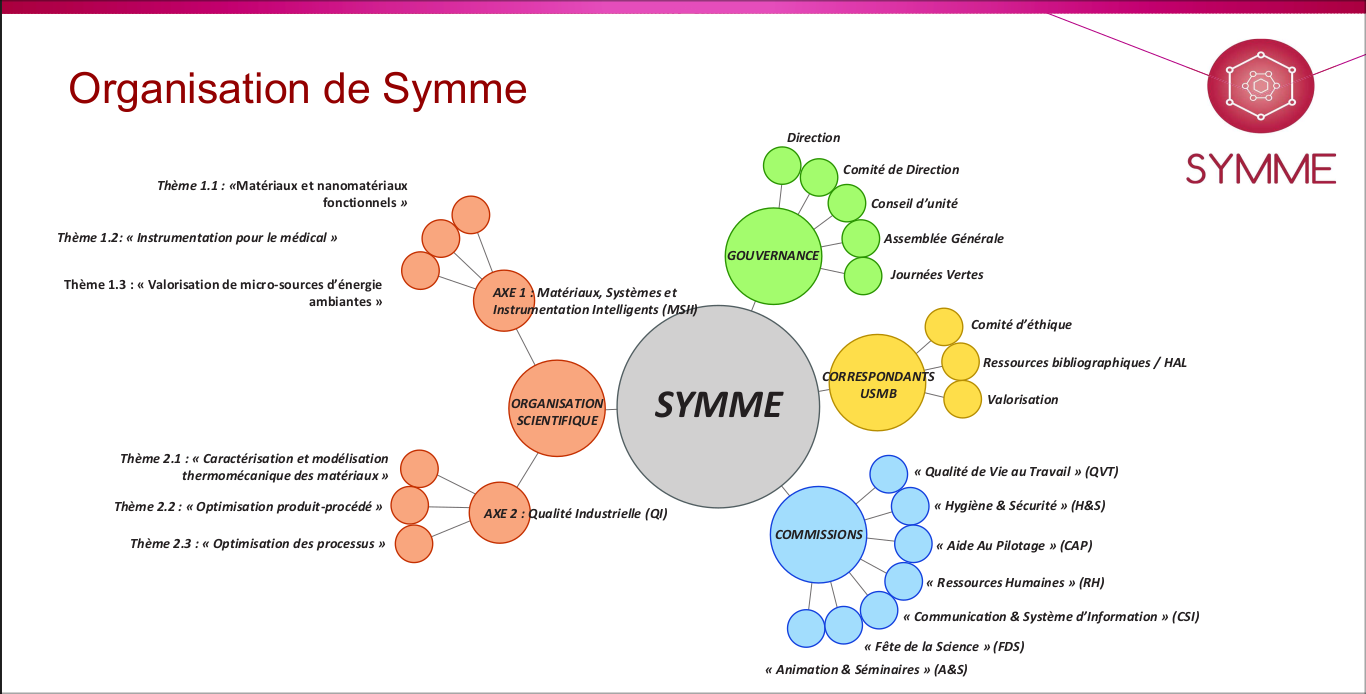
\includegraphics[width=\linewidth]{organigramme.png}
  \caption{Organisation du laboratoire SYMME}
  \label{fig:fig1}
\end{figure}


La figure \ref{fig:fig1} montre l'organisation du laboratoire SYMME. \\

C'est dans le thème "Matériaux, systèmes et instrumentation intelligents - valorisation de micro-sources d'énergies ambiantes" que s'inscrit ce stage. 

\subsection{Sujet de stage}

Le déploiement de réseaux de capteurs sans fil communicants nécessite l’utilisation de batteries qui ont une durée de vie limitée.
 Le domaine de la récupération d’énergie vibratoire vise à remplacer, ou du moins complémenter, l’usage de ces batteries au moyen de systèmes innovants de récupération et de stockage d’énergie robustes et fiables.
  Un récupérateur d’énergie vibratoire est généralement composé d’un oscillateur mécanique, de transducteurs électromécaniques (par exemple des transducteurs piézoélectriques) pour la conversion de l’énergie mécanique des vibrations en énergie électrique et d’un circuit d’extraction électrique.
   Les premiers travaux dans le domaine utilisaient des récupérateurs linéaires, c’est-à-dire, ceux composés d’un oscillateur linéaire.
    Cependant, de tels récupérateurs présentent une bande de fréquences étroite et ne sont donc pas adaptés à un environnement présentant un spectre de vibration riche et varié. 
    Une solution prometteuse pour élargir la bande de fréquences est de considérer un oscillateur non-linéaire. 
    Cependant, les comportements des récupérateurs non-linéaires sont plus difficiles à prédire de part l’existence de plusieurs solutions pour une fréquence de vibration donnée. 
    Une analyse approfondie est nécessaire pour une compréhension complète de la dynamique.
     Dans le cadre du stage, le candidat sera en charge de modéliser un récupérateur non-linéaire développé au sein du laboratoire SYMME et se familiarisera avec les outils numériques déjà mis en place.\\

L’objectif de ce stage est de développer une interface graphique pour l'analyse d'influence des paramètres du modèle. 
La dynamique pourra être visualisée sur l’interface. 
Le projet open-source sera développé en Python ou en Julia. 
Le stagiaire définira les fonctionnalités de l’application et passera à la phase de développement de l’application. 
Par exemple, il faudra faire en sorte que l’utilisateur puisse choisir un modèle de récupérateur d’énergie vibratoire, définir le type d’excitation, changer les valeurs numériques des paramètres et choisir les variables qu’il souhaite visualiser.
 Le stagiaire utilisera un outil de développement logiciel open-source de son choix (Gitlab, GitHub) afin d’assurer une intégration continue et associer une documentation (manuel d’utilisation) à l’application. 
 Durant le stage, le candidat développera ses compétences en développement logiciel et modélisation numérique.
  Il sera intégré dans une équipe ayant une expertise dans la modélisation, conception et développement de solutions pour la récupération d’énergie, au laboratoire SYMME (Annecy). 
  Selon l’avancement du stage, l’application développée par le stagiaire pourra faire l’objet d’une publication d’un article scientifique.

\newpage

\section{Contexte scientifique}


\subsection{Les récupérateurs d'énergie}

L'utilisation de récupérateurs d'énergie permet de récolter de l'énergie vibratoire.
 Il en existe de plusieurs sortes, par exemple les récupérateurs d'énergie piézoélectriques linéaires, qui peuvent amplifier les vibrations s'ils sont excités à leur fréquence naturelle. 
 Ceci dit, ces récupérateurs d'énergie ne peuvent récupérer une puissance importante qu'au sein d'une bande passante très étroite.
  Les récupérateurs d'énergie vibratoire non linéaires ont une bande passante bien plus large, bien que la complexité de leurs comportements puisse les rendre difficiles à analyser. \\

Les récupérateurs d'énergie non linéaires multi-stables peuvent présenter plusieurs cycles limites stables, appelés orbites, qui dépendent des conditions initiales et de la fréquence de vibration.
 Certaines de ces orbites, appelées orbites hautes, correspondent à un mouvement oscillatoire entre deux positions stables de la masse inertielle.
  D'autres, appelées orbites basses, correspondent à une situation où la masse inertielle oscille faiblement autour d'une seule position stable.
   Les orbites hautes sont beaucoup plus intéressantes pour la récupération d'énergie, parce qu'elles représentent une puissance plus importante. 
   Les équations différentielles du système permettent de déterminer les différentes orbites cohabitant sur une fréquence donnée, mais aussi la stabilité desdites orbites grace à une simulation.
    La détermination de si une orbite est une sous-harmonique, et de son ordre, permet une classification de celles-ci en fonction de la puissance attendue. \\

Les orbites hautes sont beaucoup plus intéressantes pour la récupération d'énergie, et la puissance récupérée augmente avec la fréquence, alors que l'inverse est vrai pour les orbites basses.
 Ainsi, pour les fréquences où différentes orbites basses et hautes cohabitent, il est intéressant de mettre en place une stratégie de saut d'orbite afin de forcer l'oscillateur à se positionner sur une orbite haute et récupérer plus d'énergie [1]. \\


\subsection{Les sauts d'orbite}

Le but d'un saut d'orbite est de forcer un oscillateur à passer d'une orbite basse à une orbite haute, et ce en dépensant le moins d'énergie possible. 
Il existe différentes manières d'effectuer cette manipulation, par exemple en donnant une impulsion venant perturber la trajectoire de la masse, ou encore en utilisant un bruit blanc [2]. 
Une autre méthode consiste à modifiant certains paramètres de l'oscillateur.
 Il est important de trouver la méthode la moins coûteuse en énergie afin que le système reste rentable. \\

Pour un oscillateur bistable de Duffing, cinq paramètres jouent un rôle important dans son comportement : la masse M, la raideur k, la valeur des positions stables $x_0$, la longueur L et l'amortissement µ. 
Notons que le niveau de flambement, donné par $\frac{x_0}{L}$, sera indirectement modifié par la modification d'autres paramètres. 
Ainsi, en modifiant l'un de ces paramètres, il est possible d'augmenter l'énergie potentielle du système et ainsi le faire passer d'une orbite basse à une orbite haute. \\

Afin d'expérimenter ces différentes stratégies, l'équipe de recherche a mis en place un prototype d'oscillateur bistable à ensemble masse-ressort flambé, permettant de modifier facilement certains de ces paramètres, et surtout d'étudier les performances d'énergie de récupération. 
Un schéma de ce prototype peut être vu en figure \ref{fig:prototype}. 
Ce système a l'avantage d'être à la fois compact et facile à mettre en place [3]. \\


\begin{figure}[H]
  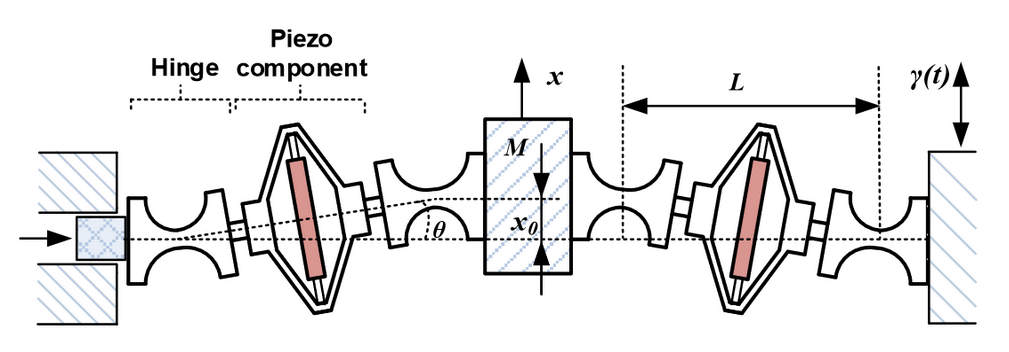
\includegraphics[width=\linewidth]{prototype.png}
  \caption{Organisation du laboratoire SYMME}
  \label{fig:prototype}
\end{figure}

C'est ce genre d'oscillateurs qui est utilisé dans le projet de recherche dans lequel s'inscrit ce stage.
 C'est donc également ce genre d'oscillateurs bistables qui sera utilisé dans les modélisations de l'application à réaliser.\\

\subsection{La place de ce stage}

Pour mettre en place une stratégie de saut d'orbite efficace, il est donc nécessaire non seulement de connaître la méthode la moins gourmande en énergie, mais également d'intervenir au meilleur moment de la trajectoire de l'oscillateur.
 La modélisation permet d'observer les comportements des oscillateurs mécaniques afin de les étudier et d'observer leurs réactions face à des perturbations ou des modifications de leurs paramètres.
  \\

La création d'une application telle que décrite dans le sujet de stage peut permettre de faire ce genre de modélisation.
 Le but est également de pouvoir observer d'autres aspects, tels que les sections de Poincaré du système, et ainsi obtenir une observation relativement diverse sur un même oscillateur. \\

Cette application pourrait également être utilisée dans un but de vulgarisation scientifique.
 En effet, son utilisation, qui se veut simple et intuitive, pourrait être une bonne illustration sur les récupérateurs d'énergie, mais aussi sur les oscillateurs mécaniques en général et tous les différents phénomènes observables sur les animations disponibles. \\



\newpage 

\section{Contenu du stage}


\subsection{Travail effectué}


Durant ce stage, différents outils de travail ont été utilisés.
 La totalité du code écrit se situe dans un repository Git, dont l'utilisation a permis de travailler en équipe, récupérer d'anciennes versions du code, et l'application finale disponible.
  La programmation a été réalisée sur l'éditeur de code Visual Studio Code, dont les extensions permettent d'utiliser de nombreux langages différents, ainsi que des outils tels que Git, de manière rapide et instinctive.
   Après plusieurs discussions, il a été décidé que la programmation serait faite en utilisant le langage Julia, plus rapide et performant que Python, et avec des librairies simplifiées sur la résolution d'équations différentielles et l'affichage de graphes interactifs. \\

Travailler sur ce sujet a impliqué d'essayer différentes librairies Julia afin de mieux se rendre compte de ce qu'il était possible de faire avec ce langage.
 Il a vite été important de savoir exactement ce que les outils intégrés à Julia permettent de réaliser comme interface graphique. 
 Pour cela, la modélisation des oscillateurs a d'abord été faite "à la main", en suivant une résolution d'équation différentielle numérique à l'aide de la méthode de Runge-Kutta d'ordre 4.
  Il s'est ensuite avéré que plusieurs paquetages Julia étaient capables de faire cette résolution de manière beaucoup plus rapide et intégrée dans différentes fonctions d'animation.
   Il existe, en Julia, une librairie de systèmes dynamiques déjà enregistrés. 
   Il est possible de créer son propre système dynamique avec les équations qui le caractérisent afin qu'il se comporte de la même manière que ceux qui ont été pré-enregistrés, ce qui est très utile car certaines fonctions d'animations intéressantes ne fonctionnent qu'avec un système dynamique en entrée. 
   Un oscillateur bistable a donc été codé de cette manière, déclaré comme système dynamique, afin de se servir de ces propriétés. 
   Cependant, la modélisation initiale a servi pour faire différents essais d'interface graphique. \\


\subsubsection{Interface graphique}

Il est vite devenu apparent que le paquetage \emph{Gtk.jl} permettait de créer des interfaces graphiques interactives assez facilement.
 La création de curseurs pour modifier les paramètres et de menus déroulants pour changer de condition initiale a été étudiée afin de faire une fenêtre permettant de modifier un graphique.
  Les graphiques ont été codés à l'aide de du paquetage \emph{Plots.jl}.
   L'utilisation de macros permettent de créer des GIFs ou des animations en seulement une ligne de code. 
   Ces différentes fonctionnalités ont été utilisées pour réaliser une première fenêtre interactive. 
   Cette première fenêtre simule la trajectoire d'un oscillateur répondant à l'équation $\ddot x = - \delta * \dot x - \alpha * x - \beta * x^3 + t $ de deux manières : à gauche, un graphe statique, et à droite un gif dynamique du même graphe. 
   Sur le graphe de droite, le tracé bleu représente exactement la même trajectoire que sur le graphe de gauche, et le tracé orangé représente un oscillateur avec les mêmes paramètres, mais dont les conditions initiales sont différentes et peuvent être redéfinies par le menu déroulant juste au-dessus, sur la droite de la fenêtre. 
   À gauche de ce menu déroulant se trouvent trois curseurs correspondant respectivement aux paramètres $\alpha$, $\beta$ et $\delta$. \\

La figure \ref{fig:interactive1} est une vue classique de cette fenêtre, c'est ce que l'utilisateur peut voir à l'exécution du code.\\

\begin{figure}[H]
  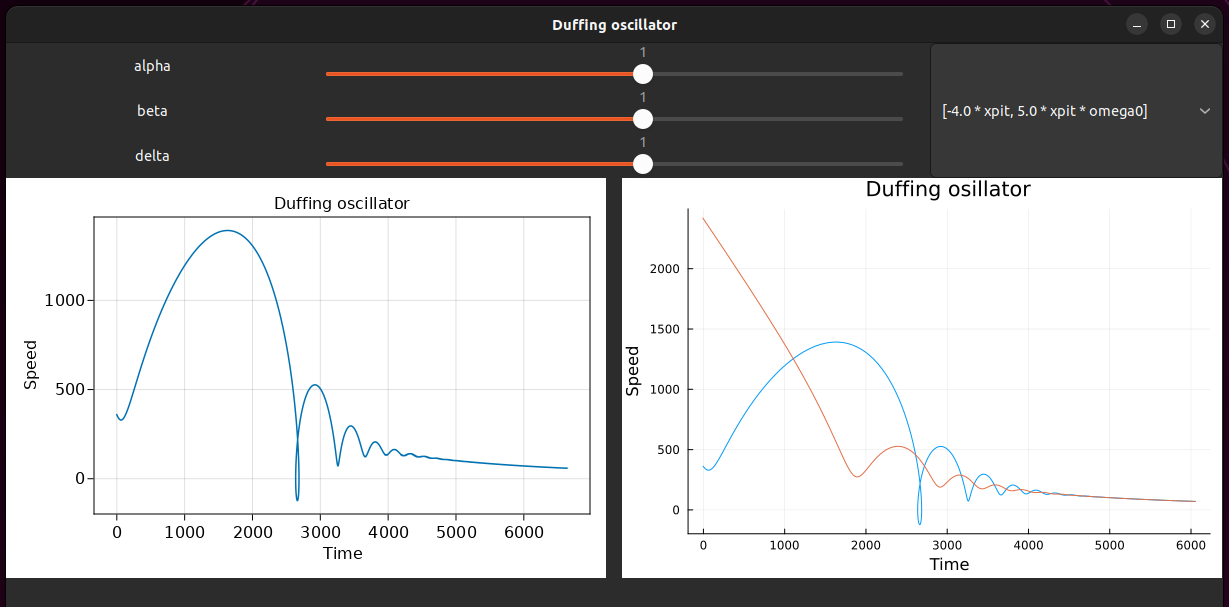
\includegraphics[width=\linewidth]{interactivewindow_1.png}
  \caption{Vue classique de la fenêtre interactive créée avec le paquetage \emph{Gtk.jl}}
  	\label{fig:interactive1}
\end{figure}


La figure \ref{fig:fig3} permet d'illustrer le mouvement du graphe de droite : la capture a été prise à un moment où le graphe n'est pas encore complet. 
Ce graphe se crée en boucle : une fois arrivé à la fin du temps pris pour la trajectoire, il s'efface et recommence. \\
\\

\begin{figure}[htb]
  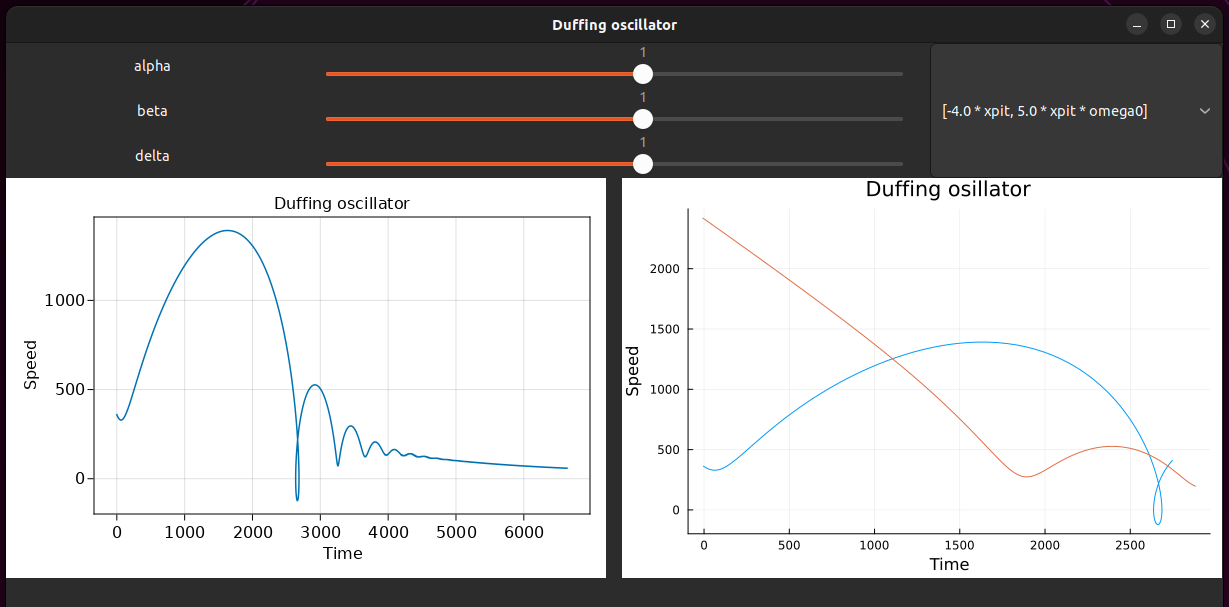
\includegraphics[width=\linewidth]{interactivewindow_2.png}
  \caption{Vue de la fenêtre interactive avec le gif pris à un autre moment}
  \label{fig:fig3}
\end{figure}


Les curseurs permettent de modifier les paramètres de l'équation différentielle et voir leur impact immédiatement sur les graphes. 
La figure \ref{fig:fig4} donne une vue de la fenêtre interactive avec l'un des paramètres modifiés. \\


\begin{figure}[H]
  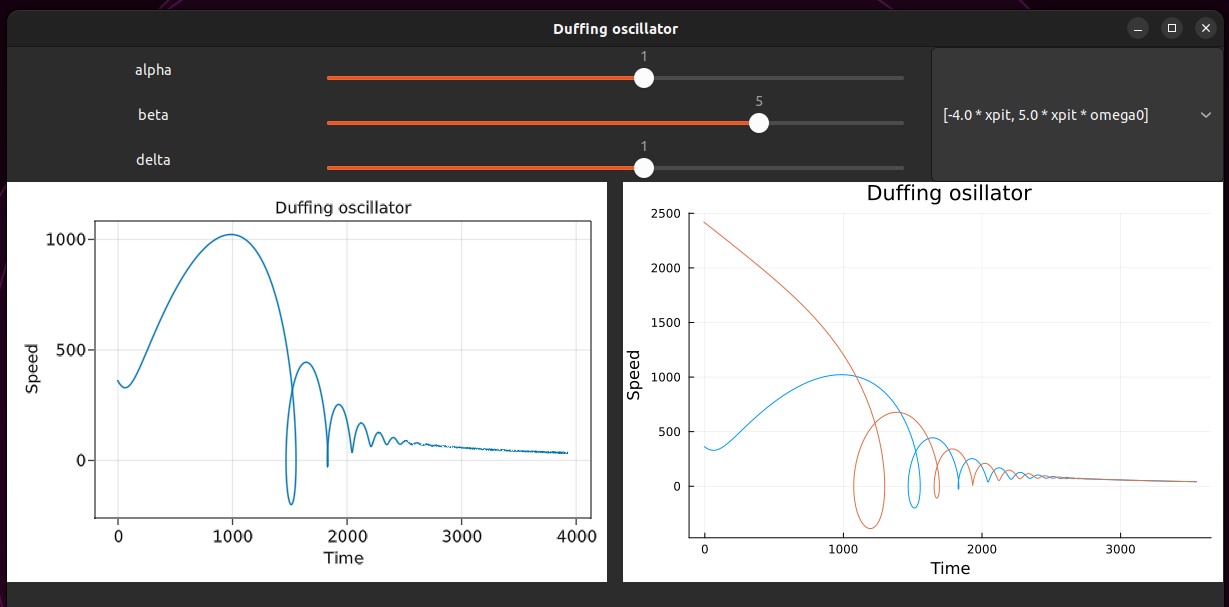
\includegraphics[width=\linewidth]{interactivewindow_3.png}
  \caption{Vue de la fenêtre interactive avec des paramètres différents}
  \label{fig:fig4}
\end{figure}


Le menu déroulant en haut à droite de la fenêtre permet de modifier les conditions initiales du tracé orange sur le graphe de droite. 
La figure \ref{fig:fig5} montre ce qu'une modification de ces conditions initiales donne. \\

\begin{figure}[H]
  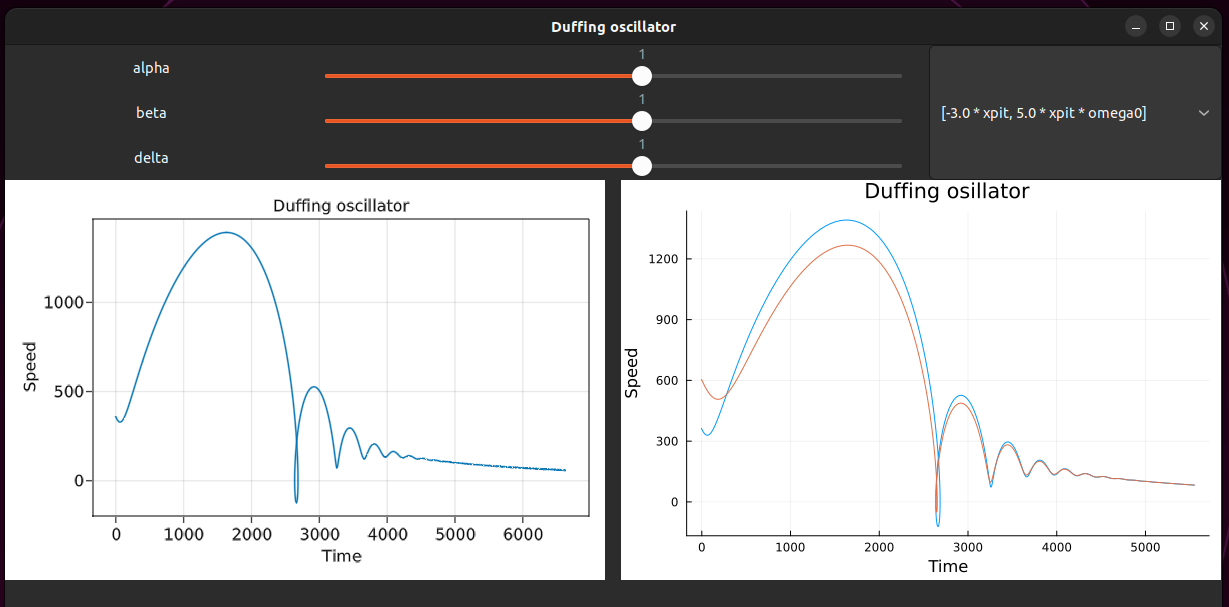
\includegraphics[width=\linewidth]{interactivewindow_4.png}
  \caption{Modification des conditions initiales pour le tracé orange}
  \label{fig:fig5}
\end{figure}

Une autre façon de créer des interfaces graphiques en Julia est d'utiliser l'extension Visual Studio Code \emph{Génie Builder}. 
Cette extension permet d'organiser une fenêtre graphique avec un système de "cliqué-glissé" qui se construit automatiquement en générant un code html.
 Il est ainsi possible de mettre en place tous les éléments souhaités (graphes, boutons, curseurs, menus déroulants... mais aussi textes interactifs, par exemple) de manière intuitive et rapide. 
 À condition de maîtriser l'outil, cela peut permettre de gagner beaucoup de temps pour le côté purement graphique de l'application. 
 Un fichier \emph{app.jl} contient le code de l'application en elle-même, c'est-à-dire le code des modélisations, calculs et autres programmations nécessaires.
  Il faut ensuite créer des variables spécifiques contenant, par exemple, le résultat d'un calcul.
   Ces variables-la communiquent avec l'interface.
    Dans l'onglet qui sert à créer l'interface par système de cliqué-glissé, il suffit de sélectionner un élément mis en place afin d'en modifier certaines caractéristiques, notamment quelles sont les valeurs ou actions qui lui sont associées. \\

La figure \ref{fig:fig6} montre la fenêtre de travail de l'extension \emph{Génie Builder}.
C'est une fenêtre générée automatiquement lors de la création d'une nouvelle application.
 Sur la droite, sous la catégorie "Bindings", se trouvent toutes les variables permettant de communiquer entre l'interface et le code du fichier \emph{app.jl}. 
 Sur l'interface de travail, le graphique (dernier élément, en bas) est sélectionné.
  Dans la colonne de droite, il est possible d'en modifier les propriétés, par exemple les valeurs prises dans le champ "Data". \\

\begin{figure}[H]
  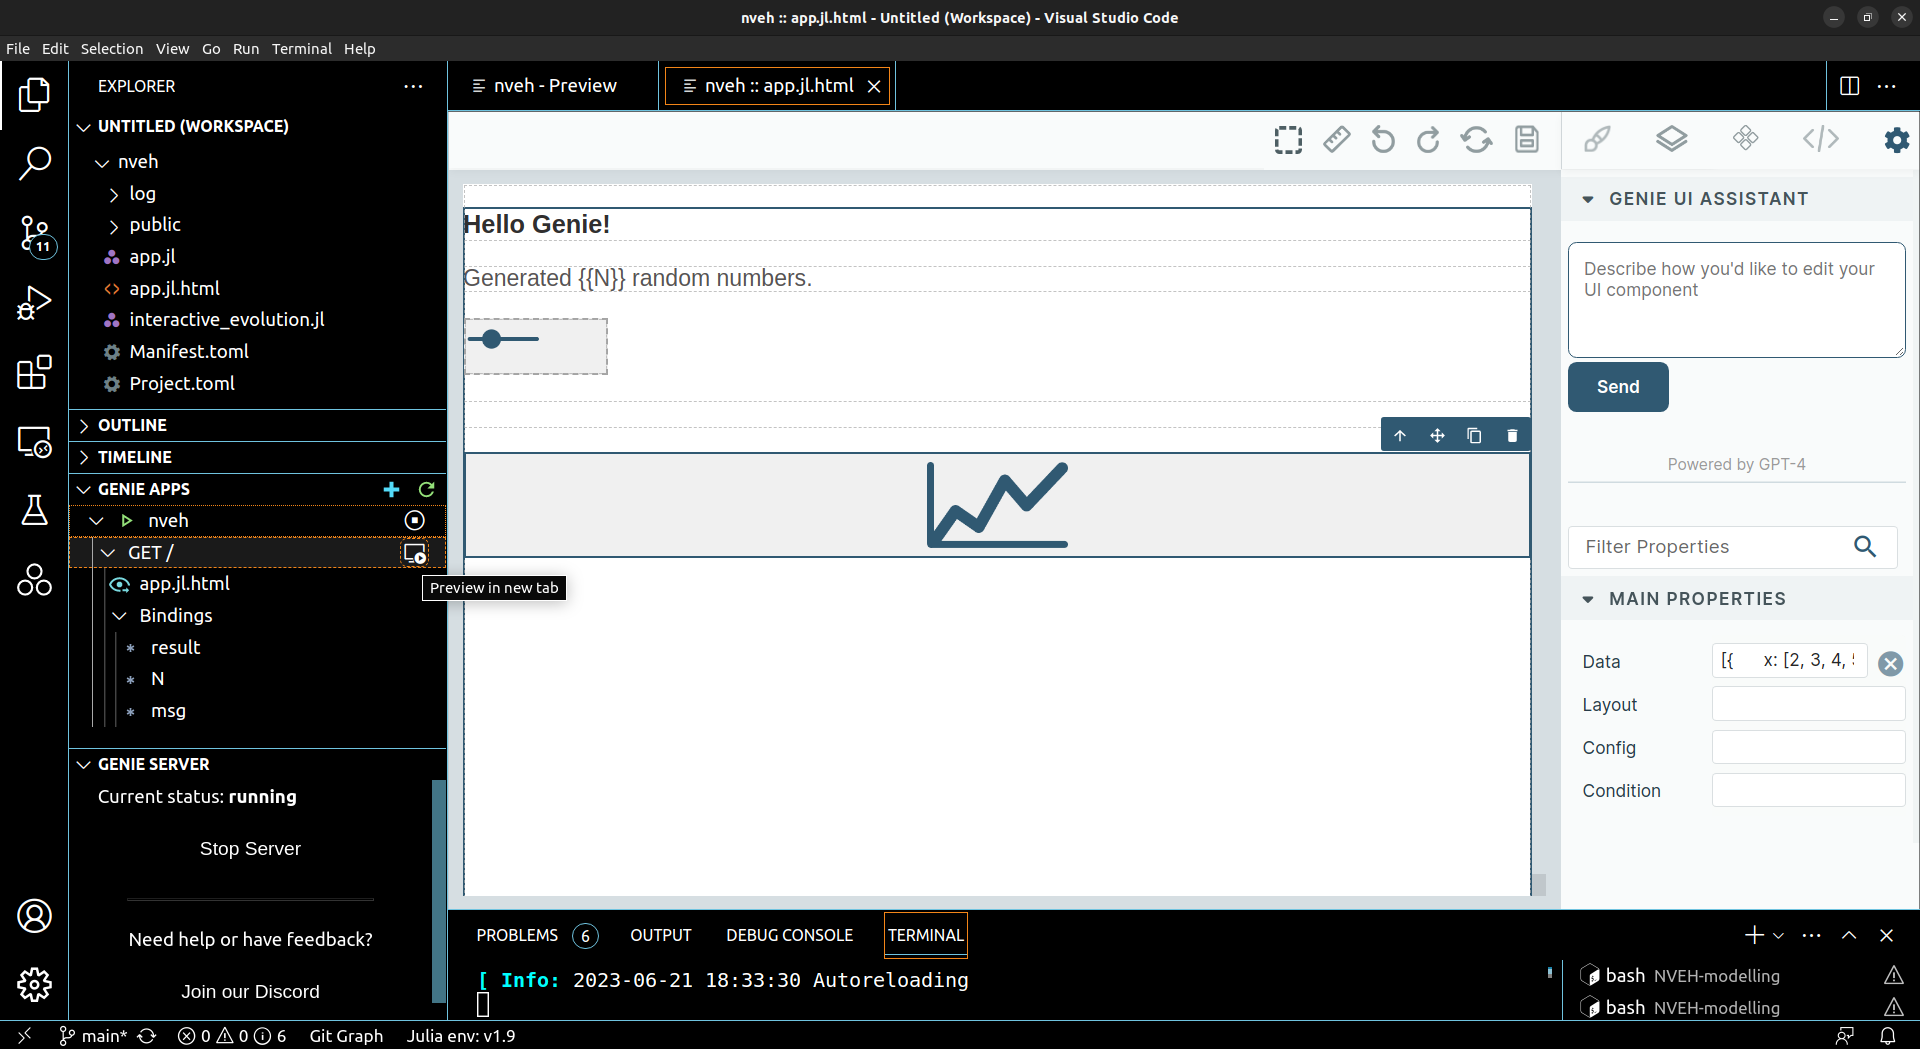
\includegraphics[width=\linewidth]{geniebuilder_travail.png}
  \caption{Fenêtre de travail de \emph{Génie Builder}}
  \label{fig:fig6}
\end{figure}

La figure \ref{fig:fig7} montre l'aperçu de la fenêtre générée par le code de la figure \ref{fig:fig6}. 
Le curseur, interacif, et les deux messages qui se modifient lorsque le curseur est bougé, y sont présents, ainsi que le graphe avec les valeurs vues plus haut. \\

\begin{figure}[H]
  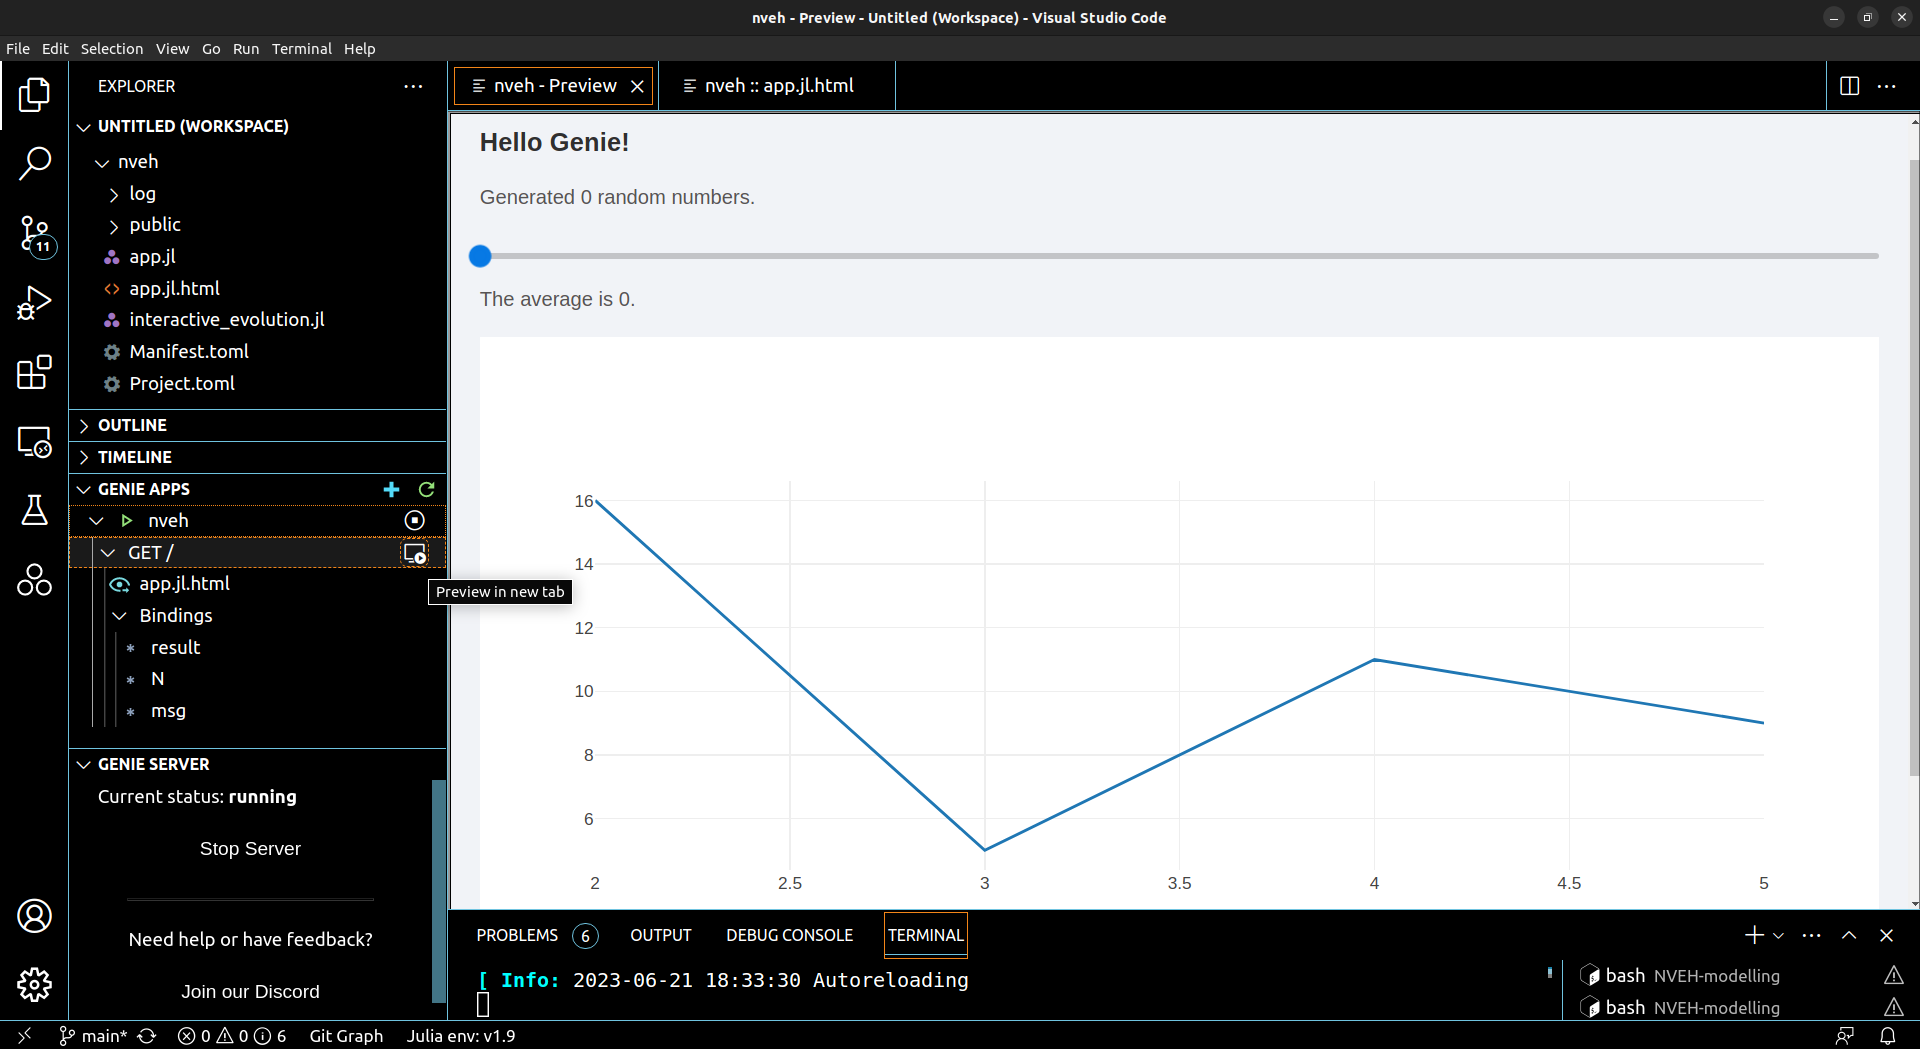
\includegraphics[width=\linewidth]{geniebuilder_result.png}
  \caption{Aperçu du résultat de \emph{Génie Builder}}
  \label{fig:fig7}
\end{figure}

Ce système a été retenu comme une possibilité pour créer l'application finale car, si maîtrisé correctement, il pourrait permettre de prendre beaucoup moins de temps sur le côté esthétique pour agencer correctement l'interface, et permettre de se concentrer un peu plus le côté modélisation et programmation.  \\

\subsubsection{Systèmes dynamiques}

En Julia, il existe de nombreux paquetages permettant de manipuler des systèmes dynamiques de manière simplifiée. 
Le premier qui sera abordé ici est le paquetage \emph{HarmonicBalance.jl}.
 Ce paquetage utilise la méthode de la balance harmonique pour calculer des solutions périodiques en passant par le domaine fréquentiel.
  Ainsi, par exemple, pour un oscillateur répondant à l'équation $\ddot x(t) + \omega_0^2 x(t) + \alpha x(t)^3 + \eta x(t)^2 \dot x (t) = F \cos(\omega t)$, le calcul et l'affichage des solutions réelles donne le graphe vu en figure \ref{fig:fig8}.\\

\begin{figure}[H]
\begin{center}
  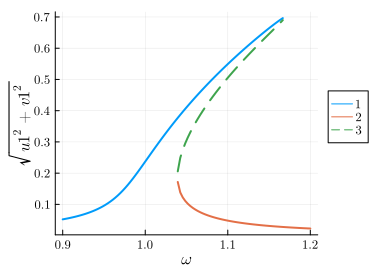
\includegraphics[width=0.45\linewidth]{harmonicbalance.png}
  \caption{Graphe montrant les solutions de l'équation calculées par la méthode de la balance harmonique}
  \label{fig:fig8}
\end{center}
\end{figure}

Pour l'obtenir, il faut déclarer l'équation différentielle étudiée ainsi que le paramètre variable souhaité en abscisse.\\

Comme vu plus tôt, Julia présente également une librairie de systèmes dynamiques déjà programmés, et il est possible de créer un objet de ce type afin d'utiliser les fonctions qui utilisent des systèmes dynamiques pour de la modélisation, par exemple. 
Ainsi, même si un système dynamique modélisant un oscillateur de Duffing existe déjà en Julia, un nouveau système a été créé afin de coller au modèle d'oscillateur bistable utilisé par l'équipe de recherche. \\

L'utilisation de la fonction \emph{interactive\_evolution()}, du paquetage \emph{InteractiveDynamics.jl}, permet de prendre en arguments un système dynamique, et de le visualiser en temps réel.
 Dans le cas présent, la trajectoire de plusieurs oscillateurs bistables, dont les conditions initiales sont définies en avance, sont visualisées. 
 La figure \ref{fig:fig9} représente l'initialisation d'une fenêtre créée ainsi. \\

\begin{figure}[H]
\begin{center} 
  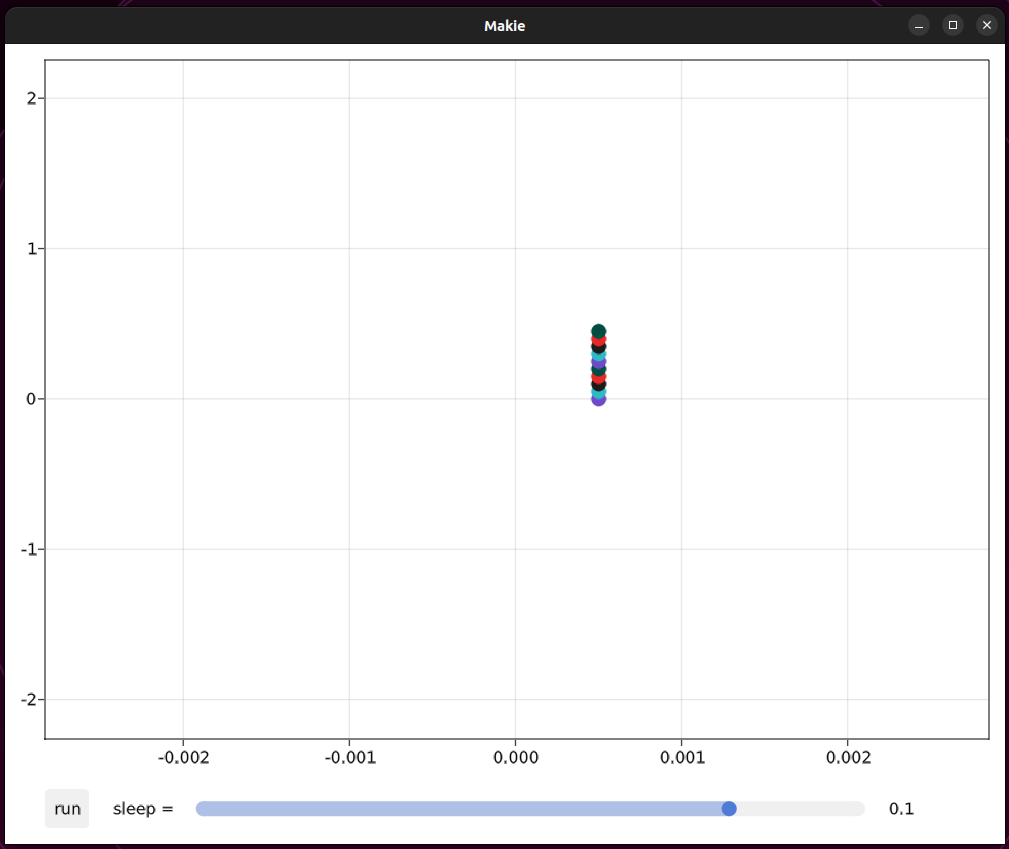
\includegraphics[width=0.8\linewidth]{interactiveevolution_0.png}
  \caption{Fenêtre initiale montrant l'évolution interactive d'oscillateurs}
  \label{fig:fig9}
\end{center}
\end{figure}

La figure \ref{fig:fig10} montre la même fenêtre un peu plus tard dans le temps.
 Le curseur situé en-dessous du graphique permet de gérer le temps de pause entre deux itérations. \\

\begin{figure}[H]
\begin{center}
  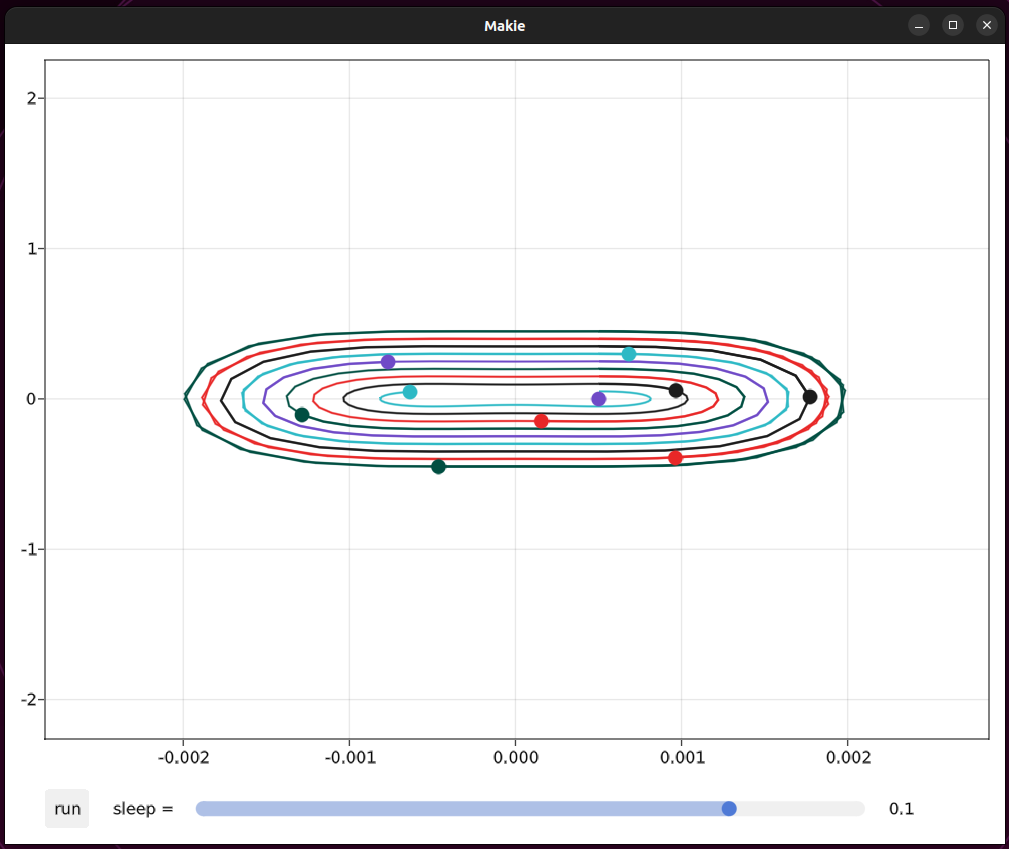
\includegraphics[width=0.8\linewidth]{interactiveevolution_1.png}
  \caption{Fenêtre montrant l'évolution interactive d'oscillateurs après quelques secondes}
  \label{fig:fig10}
\end{center}
\end{figure}

\newpage

Selon les versions du paquetage, il est possible d'entrer d'autres arguments en paramètres de la fonction \emph{interactive\_evolution()} permettant de créer des curseurs supplémentaires.
 Ces curseurs sont alors automatiquement liés à l'expression du système dynamique, et permettent de modifier des paramètres en temps réel. 
 Ce genre de fonctionnalité permet de mettre en place une visualisation comme décrite dans le sujet de stage, et ce avec un code très simple et intuitif. 
 En revanche, la version de paquetage nécessaire n'est pas compatible avec la plupart des autres paquetages ou fonctionnalités utilisées. \\

Une autre fonctionnalité utilisée permet de faire un scan en trois dimensions des sections de Poincaré d'un système.
 À nouveau, son utilisation est très simple, puisqu'il suffit de définir le système dynamique étudié et lancer la fonction \emph{brainscan\_poincaresos()}.
  Le résultat est une fenêtre interactive, avec sur la gauche une vision globale montrant la surface étudiée, sur la droite la surface de Poincaré scannée, et en bas un curseur permettant de modifier la position de la surface en question.
   Les figures \ref{fig:fig11} à \ref{fig:fig14} montrent ces résultats, avec différentes positions de la surface scannée. \\


\begin{figure}[H]
\begin{center}
  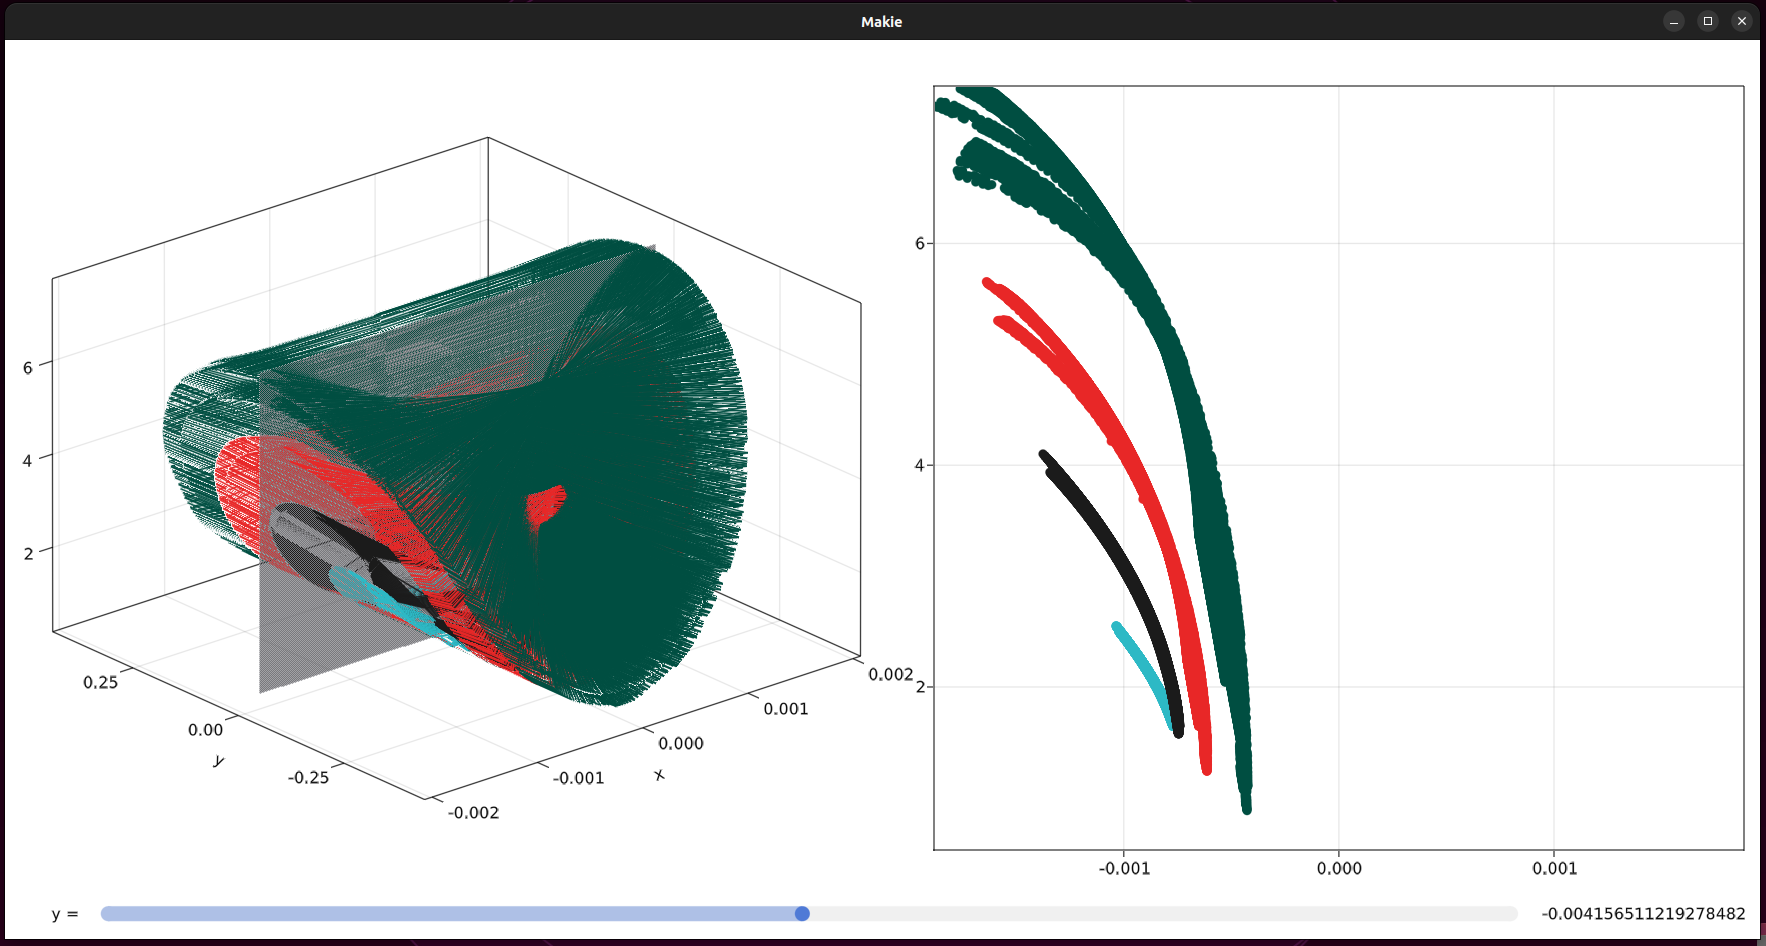
\includegraphics[width=\linewidth]{poincarescan_0.png}
  \caption{Scan des surfaces de Poincaré dans une première position}
  \label{fig:fig11}
  \end{center}
\end{figure}

\begin{figure}[H]
\begin{center}
  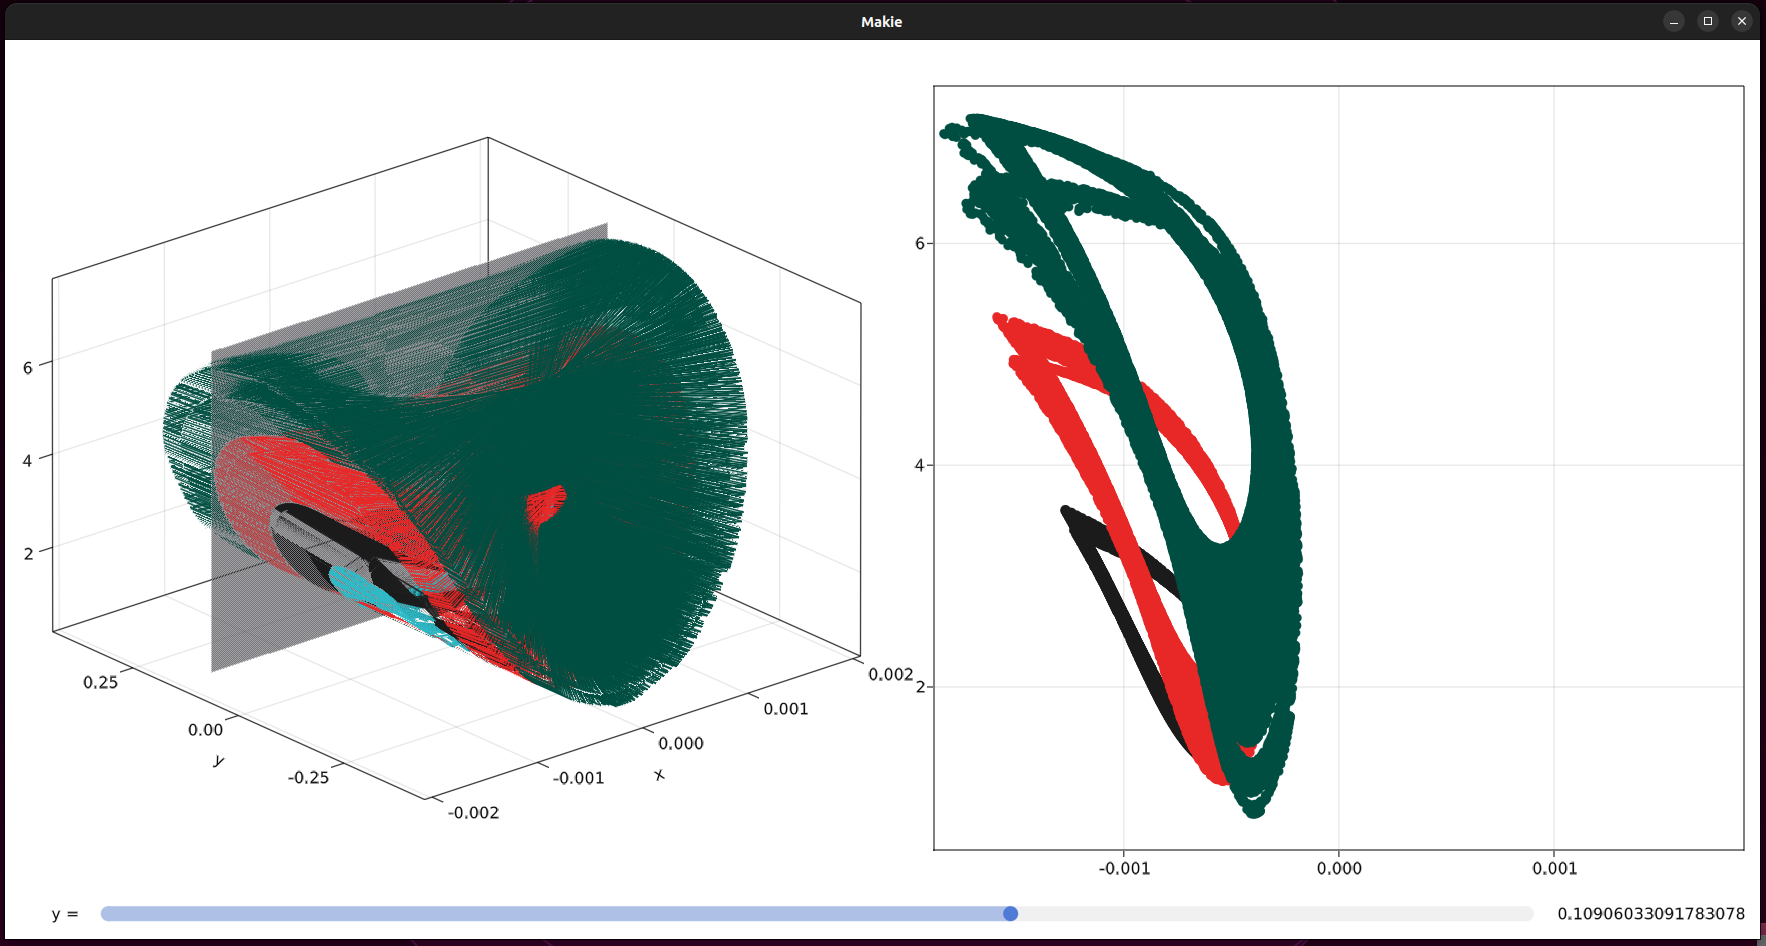
\includegraphics[width=\linewidth]{poincarescan_1.png}
  \caption{Scan des surfaces de Poincaré dans une deuxième position}
  \label{fig:fig12}
  \end{center}
\end{figure}

\begin{figure}[H]
  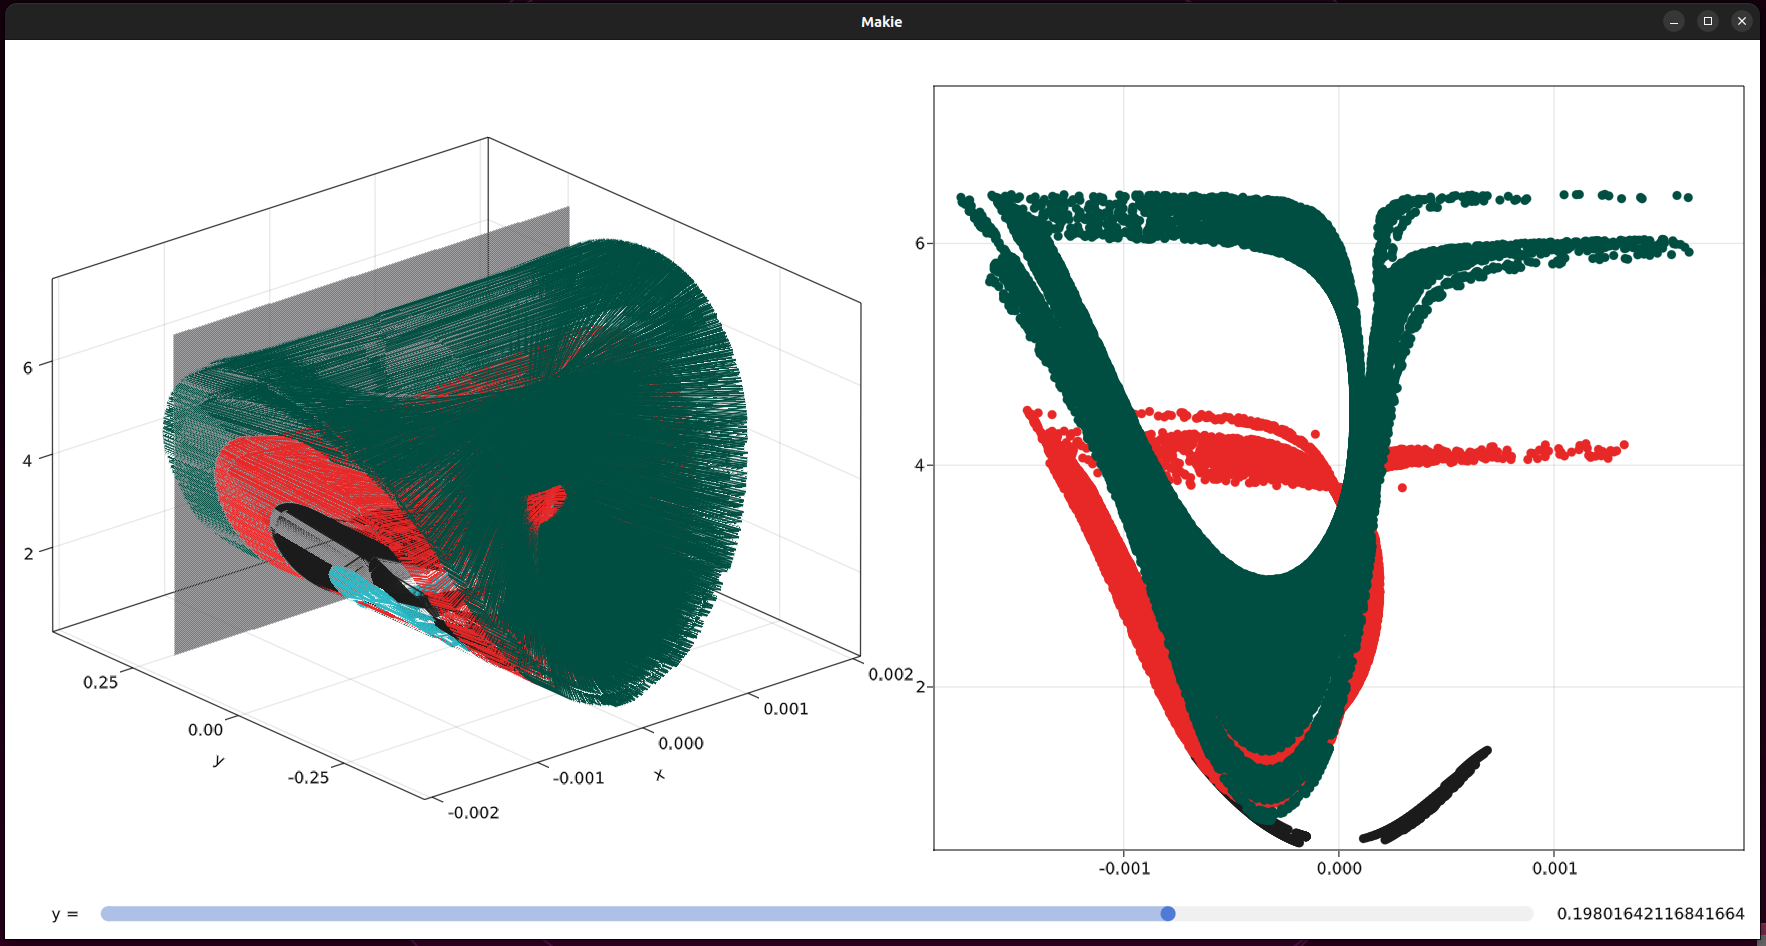
\includegraphics[width=\linewidth]{poincarescan_2.png}
  \caption{Scan des surfaces de Poincaré dans une troisième position}
  \label{fig:fig13}
\end{figure}

\begin{figure}[H]
  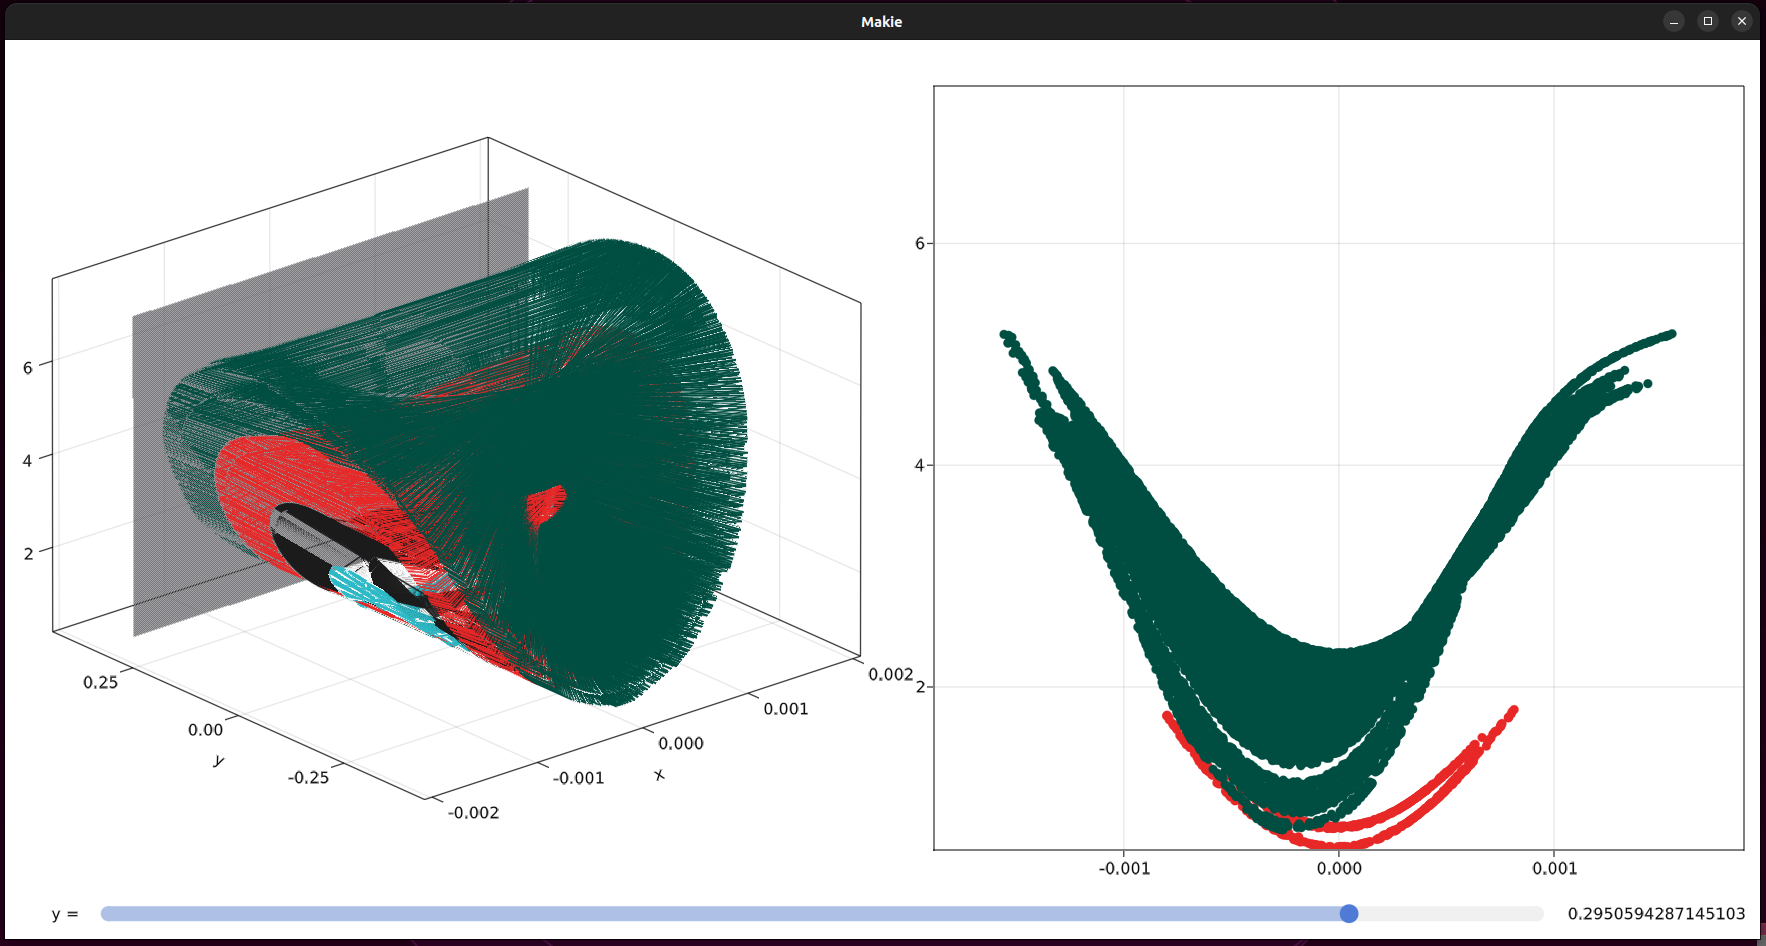
\includegraphics[width=\linewidth]{poincarescan_3.png}
  \caption{Scan des surfaces de Poincaré dans une quatrième position}
  \label{fig:fig14}
\end{figure}



Pour rester sur le thème des sections de Poincaré, une autre animation intégrée dans le paquetage \emph{DynamicalSystems.jl} permet de créer une carte interactive pour explorer une section de surface de Poincaré. 
La création de la fenêtre utilise les conditions initiales définies dans le code, et affiche toutes les solutions du système. 
Il suffit de cliquer sur un endroit du graphe pour créer de nouvelles conditions initiales et observer les solutions.
 Deux curseurs permettent de définir le temps de simulation et la taille des points.
  Les figures \ref{fig:fig15} à \ref{fig:fig18}, pages \pageref{fig:fig15} à \pageref{fig:fig18}, montrent différentes configurations de cette fenêtre, avec différentes conditions initiales créées et un exemple de taille de points plus large. \\



\begin{figure}[H]
\begin{center}
  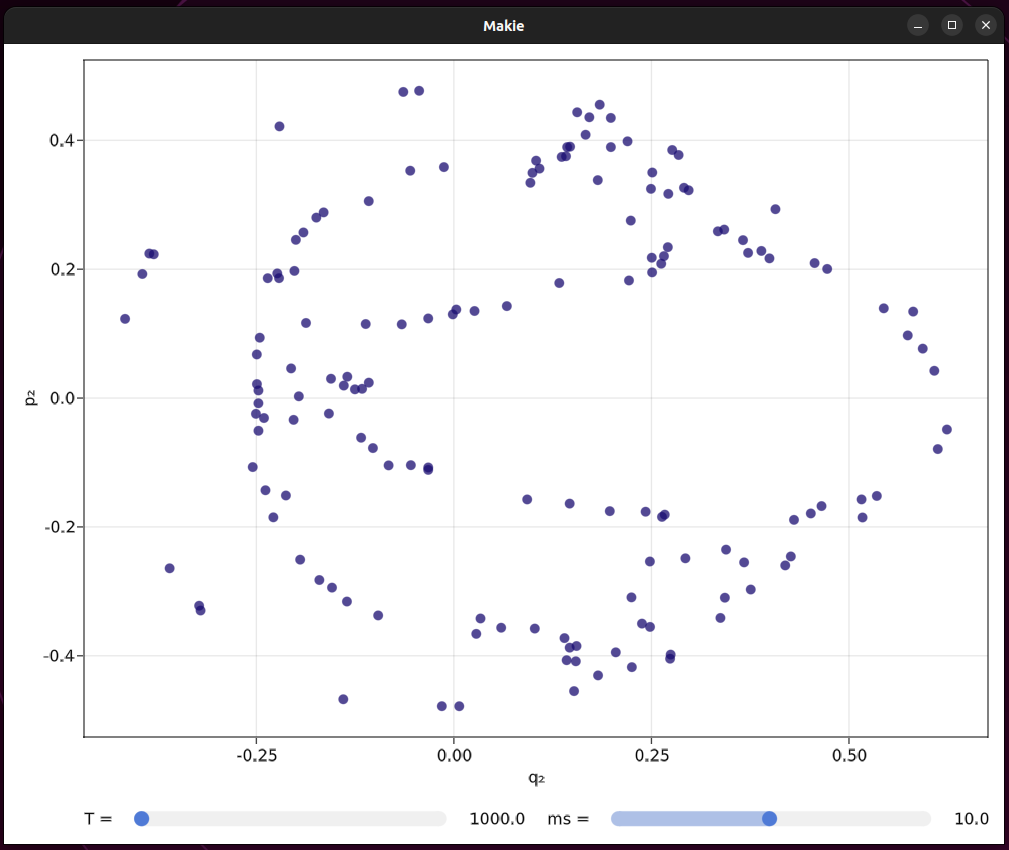
\includegraphics[width=0.7\linewidth]{poincaremap_0.png}
  \caption{Fenêtre initiale de la carte des surfaces de Poincaré interactive}
  \label{fig:fig15}
  \end{center}
\end{figure}

\begin{figure}[H]
\begin{center}
  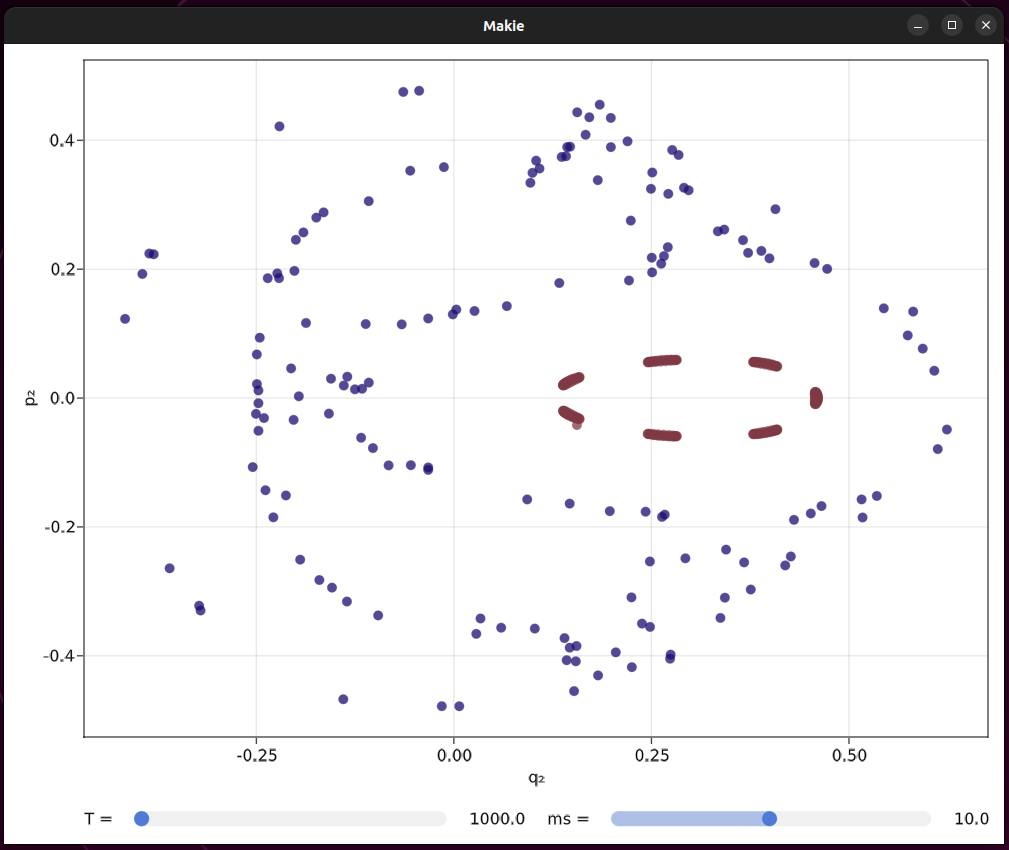
\includegraphics[width=0.7\linewidth]{poincaremap_1.png}
  \caption{Carte des surfaces de Poincarré avec une condition initiale supplémentaire}
  \label{fig:fig16}
  \end{center}
\end{figure}


\begin{figure}[H]
\begin{center}
  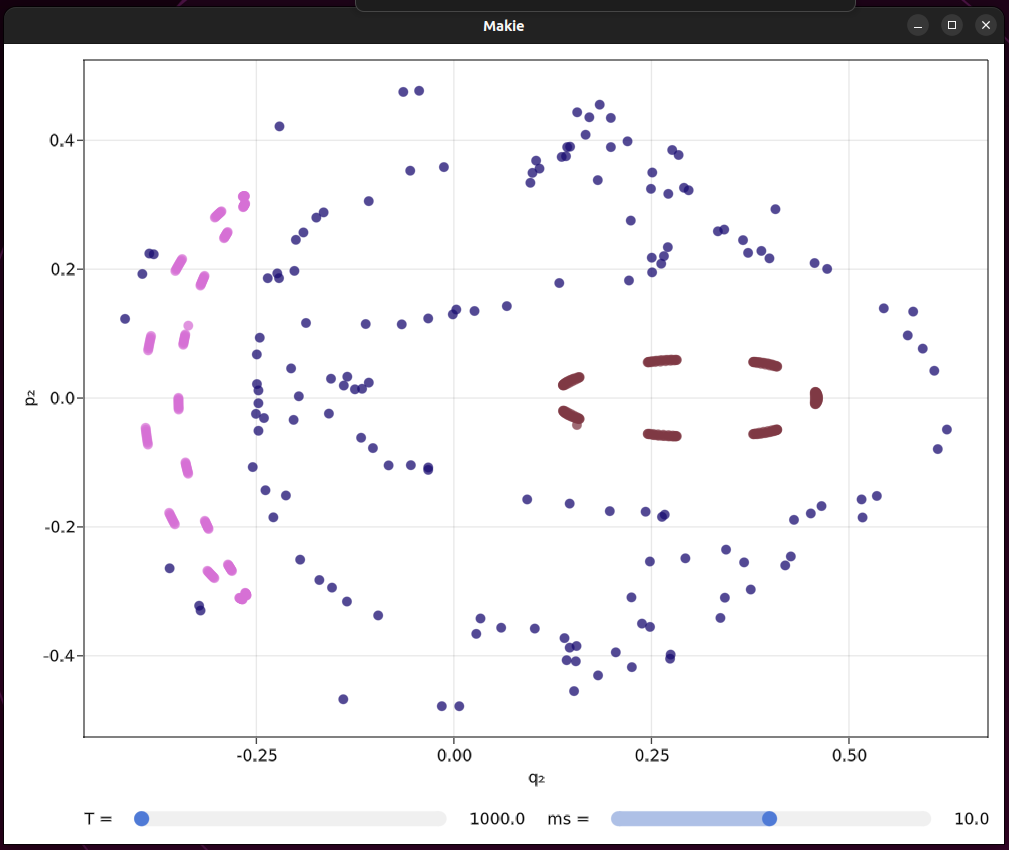
\includegraphics[width=0.7\linewidth]{poincaremap_2.png}
  \caption{Carte des surfaces de Poincaré avec deux conditions initiales supplémentaires}
  \label{fig:fig17}
  \end{center}
\end{figure}


\begin{figure}[H]
\begin{center}
  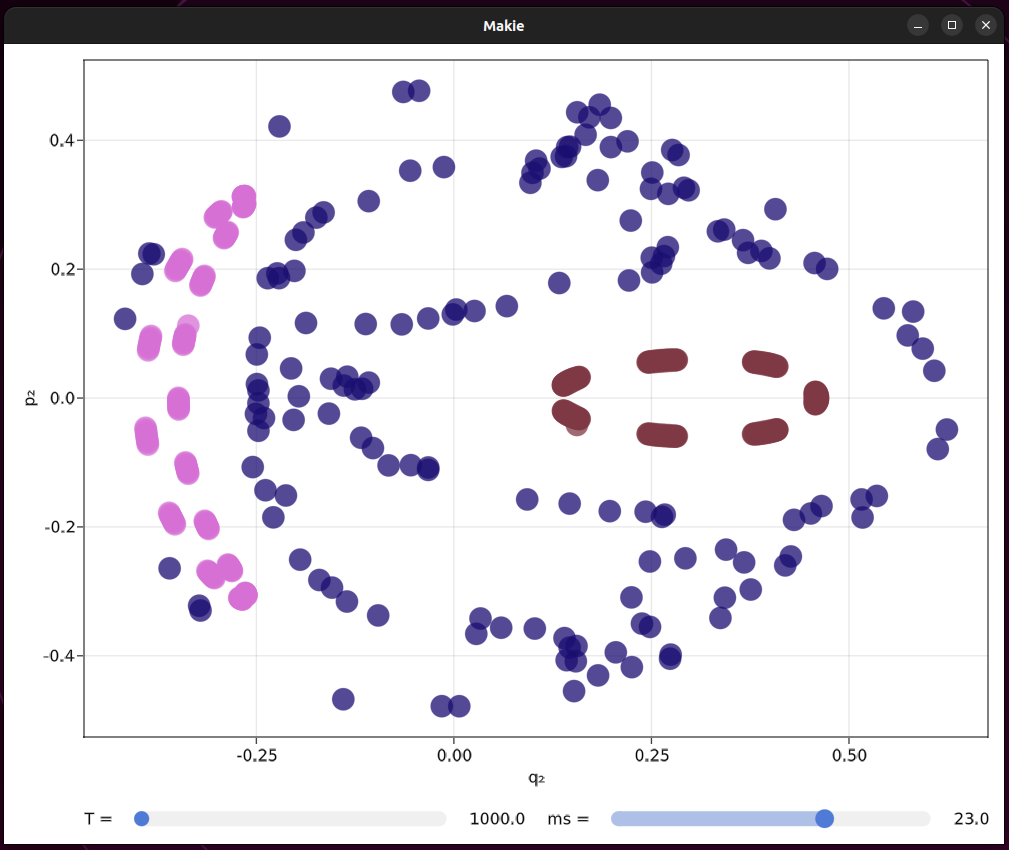
\includegraphics[width=0.7\linewidth]{poincaremap_3.png}
  \caption{Aperçu de la carte des surfaces de Poincaré avec un affichage différent}
  \label{fig:fig18}
  \end{center}
\end{figure}


 Cette animation utilise non pas un oscillateur bistable comme vu précédemment, mais un système de Hénon Heiles, qui était l'exemple pris dans l'explication de la fonction.
  Le fonctionnement avec un système bistable défini par l'équipe de travail n'a pas encore été mis en place. 
  Un système de Hénon-Heiles représente le mouvement non linéaire d'une étoile autour d'un centre galactique. \\

Ces différentes animations sont très intéressantes pour le développement de l'application désirée, car elles permettent de modéliser et afficher des résultats rapidement, avec un effort minimal. 
Elles ne sont, en revanche, pas forcément toutes compatibles avec les systèmes de création d'interfaces vus plus haut, puisqu'elles ne peuvent pas être intégrées directement dedans, et que les différentes versions nécessaires ne sont pas forcément compatibles entre elles. 


\subsection{Ce qu'il reste à faire}

Afin de pouvoir utiliser des animations qui requièrent des versions de paquetages incompatibles les unes avec les autres, il a été décidé de faire une interface principale sur laquelle l'utilisateur pourrait décider quelle animation observer. \\

Le choix d'une animation spécifique se ferait à l'aide d'un clic sur un bouton.
 C'est ce clic qui pourrait commander la lecture du fichier contenant le code de l'animation en question. 
 En haut de ce fichier, la commande \emph{@quickactivate()} pourrait permettre d'activer un environnement spécifique de Julia, contenant les versions de paquetage nécessaires au fonctionnement de l'animation souhaitée.
  Il faut donc mettre en place les différents environements nécessaires, et terminer de créer les animations afin de répondre au cahier des charges.
   Par exemple, la carte de Poincaré interactive n'est pas encore codée pour utiliser un oscillateur bistable correspondant à celui utilisé par l'équipe de recherche. \\

Pour ce qui est de la fenêtre principale, elle sera probablement réalisée à l'aide du paquetage \emph{Gtk.jl}. 
Un essai a été fait avec l'extension \emph{Génie Builder}, mais l'intégration du fichier contenant l'animation se faisait mal : l'enregistrement du fichier lançait l'animation, et le clic sur le bouton renvoyait une erreur. 
Probablement qu'il est possible de le faire tout de même, mais le temps dépensé à trouver la solution risque de ne pas être rentable par rapport à celui gagné pour l'agencement des différents composants de la fenêtre. 
En effet, si la fenêtre principale ne contient que quelques explications et des boutons, mais pas ou peu d'animations, l'expérience déjà acquise permettra de la réaliser rapidement, et l'aide d'une interface par cliqué-glissé devient négligeable.
 De plus, l'extension \emph{Génie Builder} a été peu utilisée jusqu'à maintenant, et n'est pas encore maîtrisée. \\

À présent que tous les éléments permettant de créer l'application sont connus, il ne reste donc plus qu'à finir de mettre en place correctement les animations et faire le lien entre elles et la fenêtre graphique principale.
 Si un cahier des charges a été établi, il a été fait avant de savoir exactement ce que Julia permettrait de réaliser. 
 Il faudra donc vérifier au fur et à mesure de l'avancement ce que l'ensemble de l'équipe souhaite mettre en place précisément dans l'application. 

\newpage 

\section{Conclusion}

La réalisation de ce stage a été une occasion d'apprendre le langage Julia et d'acquérir de nouvelles compétences en gestion de projet et en informatique. 
Si l'application n'est pas encore terminée au moment de la rédaction de ce rapport, le temps conséquent passé à explorer les différents outils mis à disposition par Julia et ses nombreux paquetages a permis d'avoir une idée assez claire du chemin qu'il reste à parcourir. \\

À présent que la création d'interfaces graphiques, de graphes interactifs, et les animations pré-programmées dans les librairies Julia sont maîtrisées, il ne reste plus qu'à assembler le tout dans une application cohérente, en utilisant le système dynamique créé par l'équipe de recherche correspondant à l'oscillateur bistable étudié.
 La principale difficulté qu'il reste à surmonter est sans doute la gestion des environnements, qui a déjà posé problème plusieurs fois durant ce stage.
  Une fois cette problématique réglée, la fin du code de l'application devrait se dérouler facilement dans les deux semaines de stage qu'il reste. \\

Il est également possible que l'équipe encadrante de ce stage demande la rédaction d'un manuel d'utilisation au terme de la programmation de l'application, ce qui serait une nouvelle expérience.
 Le fait de déployer cette application de manière publique sur internet a été discuté, mais aucune décision n'a été prise pour le moment, et les moyens de le faire n'ont pas été explorés si l'utilisation de \emph{Génie Builder} est annulée. 







\newpage 

\section{Bibliographie}

[1] Saint-Martin, C., Morel, A., Charleux, L., Roux, E., Benhemou, A., \& Badel, A. (2022). Power expectation as a unified metric for the evaluation of vibration energy harvesters. Mechanical Systems and Signal Processing, 181, 109482.\\

[2] Huguet, T. (2018). Vers une meilleure exploitation des dispositifs de récupération d’énergie vibratoire bistables: Analyse et utilisation de comportements originaux pour améliorer la bande passante (Doctoral dissertation, Université de Lyon).\\

[3] Liu, W. (2014). Conception d'un dispositif de récupération d'énergie vibratoire large bande (Doctoral dissertation, Grenoble).\\

[4] Košata, J., del Pino, J., Heugel, T. L., \& Zilberberg, O. (2022). HarmonicBalance.jl : A Julia suite for nonlinear dynamics using harmonic  balance. SciPost Phys. Codebases, 6. https://doi.org/10.21468/SciPostPhysCodeb.6

\newpage

\listoffigures

\newpage

\section{Annexes}

\subsection*{A. Cahier des charges pour l'interface de visualisation des oscillateurs}


\textbf{Objectif :} Développer une interface graphique pour comprendre l'influence des paramètres d'un oscillateur mécanique

\large{Fonctionnalités générales}
\begin{itemize}
\item L'application doit être conçue pour fonctionner sur des systèmes d'exploitation variés (Windows, MacOS, Linux), avec une installation minimale nécessaire.
\end{itemize}


\large{Fonctionnalités spécifiques}

\textbf{Priorité}
\begin{itemize}
 \item L'utilisateur doit pouvoir ajuster les paramètres suivants pour chaque oscillateur : 
 \begin{itemize}
 \item amortissement
 \item raideur
 \item amplitude, fréquence de l'excitation
 \item niveau de flambement
 \end{itemize}
 \item Ces paramètres doivent pouvoir être ajustés dynamiquement, avec une visualisation en temps réel des modifications sur les trajectoires et les potentiels élastiques.
 \item L'application doit afficher les trajectoires dans le plan de phase pour chaque oscillateur.
\item L'application doit afficher la forme de l'énergie potentielle élastique pour chaque oscillateur. Leur forme doit changer en temps réel suivant les variations induites par l'utilisateur.
 \item L'utilisateur doit pouvoir zoomer et dézoomer sur le plan de phase pour une visualisation plus détaillée ou plus large.
\end{itemize}


\textbf{Analyse de l'énergie}
\begin{itemize}
\item L'application doit fournir une option pour ajouter et visualiser des quantités d'analyse telles que l'énergie totale récupérée au cours du temps et l'espérance de puissance (dans le cas de plusieurs oscillateurs, cette quantité va évoluer au cours du lancement de l'application).
\end{itemize}

\textbf{Option}
\begin{itemize}

 \item L'utilisateur doit pouvoir choisir de lancer un ou plusieurs oscillateurs simultanément.
 \item L'utilisateur peut choisir quelle variable tracée en fonction du temps ou d'un autre paramètre 
 \item Possibilité de sauvegarder les valeurs des paramètres, les puissances des orbites, l'espérance, etc... associées aux simulations numériques sous forme d'un fichier csv ou hdf5
 \item L'utilisateur pourra alors charger une configuration de paramètre sauvgardée et reprendre à partir de celle-ci (au lieu de partir des conditions par défaut définies par le concepteur)

\end{itemize}

\textbf{Livrables} 
\begin{itemize}

\item Code source de l'application
\item Documentation technique décrivant le fonctionnement interne de l'application (rapport de stage ?)
\end{itemize}


\newpage



\subsection*{B. Rapports d'avancement}

\subsubsection*{Rapport d'avancement 1 - Semaines 1 et 2}

Ceci est le premier rapport d’avancement de mon stage. Pour rappel, le sujet de mon stage est la création d’une interface graphique permettant de visualiser les comportements d’un oscillateur mécanique de façon interactive, c’est-à-dire de façon à ce que l’utilisateur puisse modifier certains paramètres et voir leur influence en temps réel. \\

	Pour commencer mon stage et me mettre dans le sujet, j’ai commencé par lire plusieurs articles me permettant de mieux comprendre les enjeux et l’intérêt de mon stage. J’ai ainsi pu me familiariser avec le principe de récupération d’énergie vibratoire et d’orbites. Pour chaque condition initiale, plusieurs cycles limites, appelés orbites, peuvent apparaître. Parmi ces orbites, certaines, appelées “orbites hautes” permettent de récupérer plus d’énergie que les autres. J’ai eu l’occasion de faire un TP sur la simulation d'oscillateurs de Duffing, qui m’a introduit plusieurs notions comme les sections de Poincaré. J’ai également utilisé ce TP pour effectuer plusieurs tests sur l’utilisation de Numba, dont j’aurai probablement à me servir afin d’accélérer les parties simulation de mon code.\\
	 
	Une fois le sujet du stage et les différentes notions bien assimilés, j’ai pu me pencher sur l’interface en elle-même. Ma tutrice de stage, Madame Camille Saint-Martin, avait déjà réalisé une interface en utilisant Python et sa librairie PyQT. Nous avons également parlé du langage Julia. Mon travail pour les jours à venir est d’essayer les deux langages pour pouvoir les comparer et décider lequel des deux sera le plus approprié. Pour ce faire, j’ai déjà commencé à me familiariser avec le langage Julia et la manière d’afficher des images, statiques ou dynamiques, et d’intégrer du code en Python (servant à la simulation) à l’intérieur.  \\
	
	J’ai créé un repository Git sur lequel je mettrai mon code. Pour l’instant, j’ai ajouté au fichier ‘tests\_julia’ mes essais sur le langage Julia. En voici le lien : https://github.com/SalsyUniate/NVEH-modelling 


\subsubsection*{Rapport d'avancement 2 - Semaines 3 et 4}

Ceci est le deuxième rapport d’avancement de mon stage. Pour rappel, le sujet de mon stage est la création d’une interface graphique permettant de visualiser les comportements d’un oscillateur mécanique de façon interactive, c’est-à-dire de façon à ce que l’utilisateur puisse modifier certains paramètres et voir leur influence en temps réel. \\

Au début de mon stage, j’avais commencé par entrer doucement dans le sujet en lisant divers papiers et en faisant un TP sur la modélisation de l’oscillateur de Duffing. \\

Durant les deux semaines qui viennent de s’écouler, j’ai eu l’occasion d’explorer le langage informatique Julia, plus performant et plus rapide que Python, et bien documenté. J’ai commencé par faire de nombreux essais pour voir ce qu’il m’était possible de faire, et ai créé une fenêtre interactive dans laquelle j’ai pu afficher des graphes, statiques ou dynamiques, et modifier des paramètres, modifications qui se répercutent directement sur les affichages en cours. Si j’ai réussi à afficher des graphes dynamiques en créant des gifs qui se jouent en boucle, nous préférerions avoir un affichage “en temps réel”, ce qui est possible avec le langage Julia mais je n’ai pas encore réussi à le mettre en place. \\

Mes objectifs pour les semaines à venir sont donc de réussir à créer un affichage dynamique en temps réel, et avancer l’application en elle-même. J’ai commencé à créer un dossier src contenant un code plus propre pour commencer l’application, mais ce n’est encore que le tout début. J’ai également découvert une extension Visual Studio Code permettant de créer des interfaces graphiques en Julia sans avoir à les coder, avec un système graphique de “drag-and-drop”. Après discussion avec ma tutrice entreprise, nous avons décidé que si l’outil est pratique, cela pourrait me permettre de gagner du temps et de me concentrer plus amplement sur le code des simulations en lui-même. J’explorerai donc ceci. \\

Voici le lien de mon repository Git, qui contient mes différents essais et mon fichier src : https://github.com/SalsyUniate/NVEH-modelling 



\subsubsection*{Rapport d'avancement 3 - Semaines 5 et 6}

Ceci est le troisième rapport d’avancement de mon stage. Pour rappel, le sujet de mon stage est la création d’une interface graphique permettant de visualiser les comportements d’un oscillateur mécanique de façon interactive, c’est-à-dire de façon à ce que l’utilisateur puisse modifier certains paramètres et voir leur influence en temps réel. \\

Durant les quatre premières semaines de mon stage, j’avais commencé par étudier l’aspect théorique du sujet en lisant différents documents et en faisant quelques essais de code en Python. Suite à cela, j’avais commencé à explorer Julia, un langage de programmation proche de Python avec de nombreuses librairies permettant de faire des modélisations et des animations facilement. En utilisant ce langage, j’avais réussi à créer des graphiques, statiques et dynamiques, interactifs, dans une fenêtre permettant de modifier en temps réel certains paramètres. \\

Ces méthodes faites « à la main » étaient lentes et ne correspondaient pas exactement à ce qui était attendu pour l’application finale. Dans les deux semaines qui viennent de s’écouler, j’ai pris connaissance de manières bien plus simples de faire un travail plus complet. Certains paquetages Julia utilisent des objets de type systèmes dynamiques pour faire des animations interactives extrêmement complètes à l'aide de fonctions déjà programmées. Il est donc très simple de mettre en place des animations complètes et intéressantes pour notre travail. La principale difficulté vient du fait que certaines de ces fonctions nécessitent des versions de paquetages qui ne sont pas toujours compatibles avec les autres. Une solution envisagée est de créer une interface principale avec des boutons menant à des animations. L’appui sur ces boutons activerait l’environnement nécessaire et permettrait ainsi à l’utilisateur d’avoir accès à de nombreuses animations différentes. \\

L’utilisation de l’outil Génie Builder a finalement été écartée. Si l’interface graphique est aussi simple, le temps gagné par le système de cliqué-glissé ne rattrapera pas le temps perdu à maîtriser l’outil. \\

Mon objectif pour les deux semaines à venir est de terminer l’application. Ces deux semaines sont les dernières de mon stage. A présent que j’ai accès à tous les outils nécessaires (interface graphique, graphiques interactifs, animations de systèmes dynamiques…) il ne me reste plus qu’à assembler le tout en respectant les indications de ma tutrice entreprise.\\
 
Pour rappel, voici le lien de mon repository Git, qui contient l’ensemble de mon code : https://github.com/SalsyUniate/NVEH-modelling 







\end{document}